\chapter{Supplementary Graphs and Tables}
\section{Supplementary Graphs}

\subsection{Winning ration plots for simple network topologies}
\label{append:wining-ratio-further-plot}
In this section, as explained in~\ref{chap:Three}, winning ratio point plots
have been conducted. These point plots can be found below.
\begin{figure}[H]
\centering
    \begin{subfigure}[t]{1\textwidth}
    \centering
        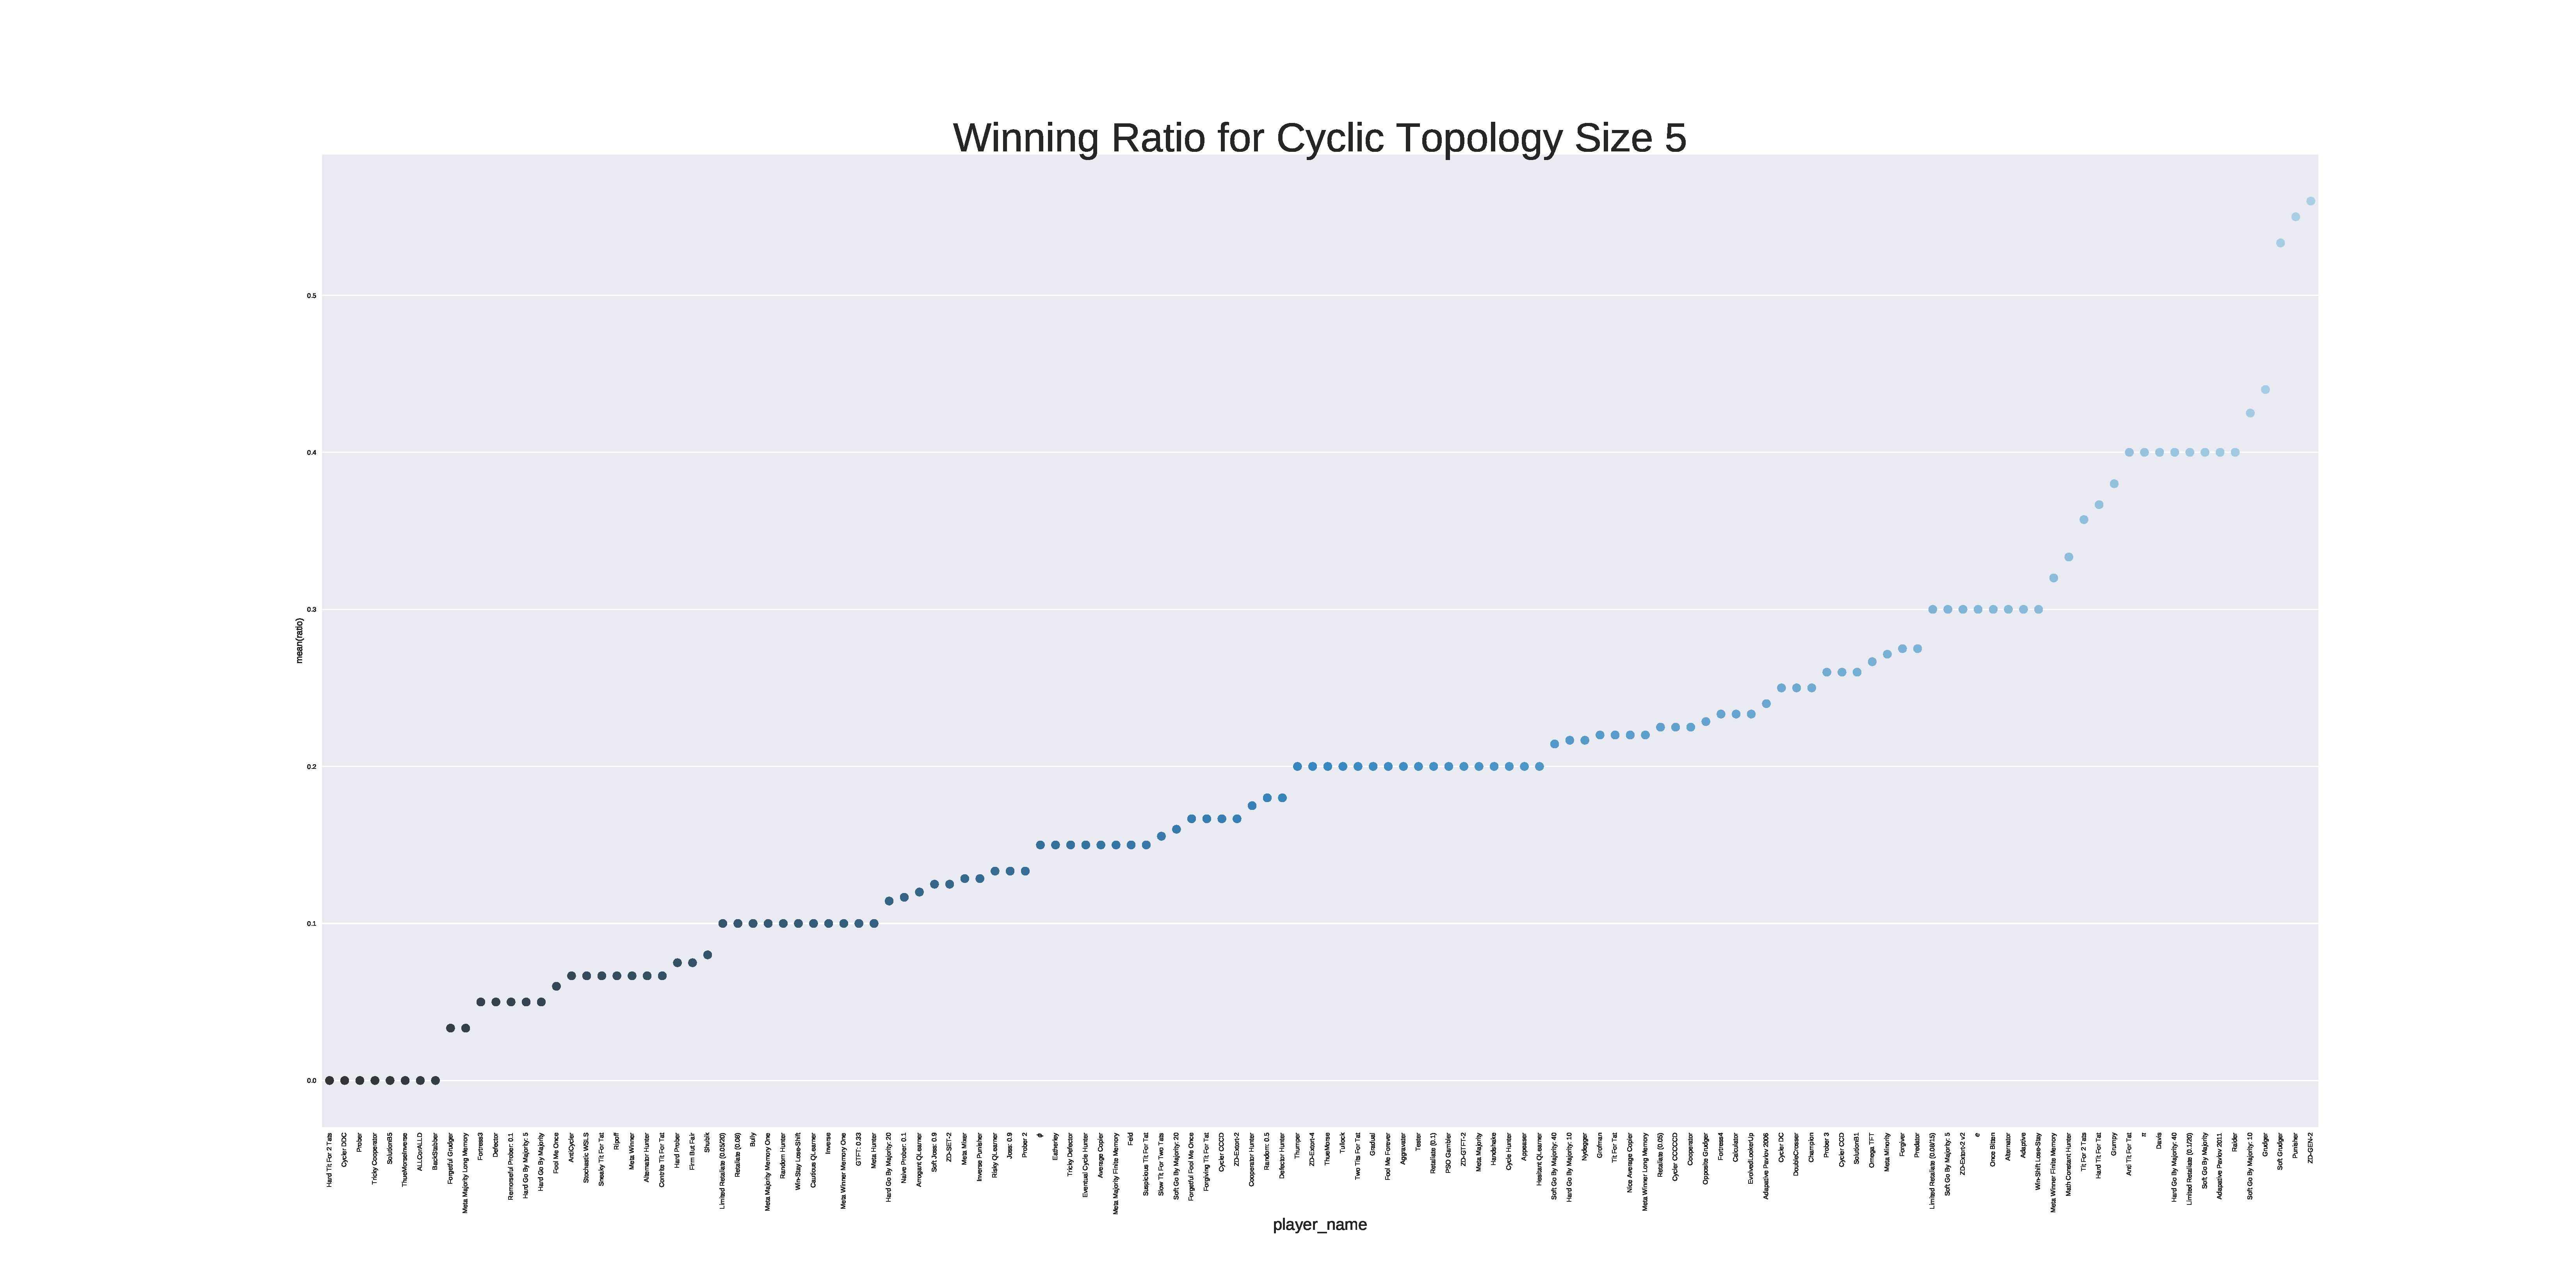
\includegraphics[width=\linewidth]{appendix/winners-Cyclic-5.pdf}
    \caption{Winning ration cycle s=5.}
    \end{subfigure}
\hfill
    \begin{subfigure}[t]{1\textwidth}\centering
    \centering
        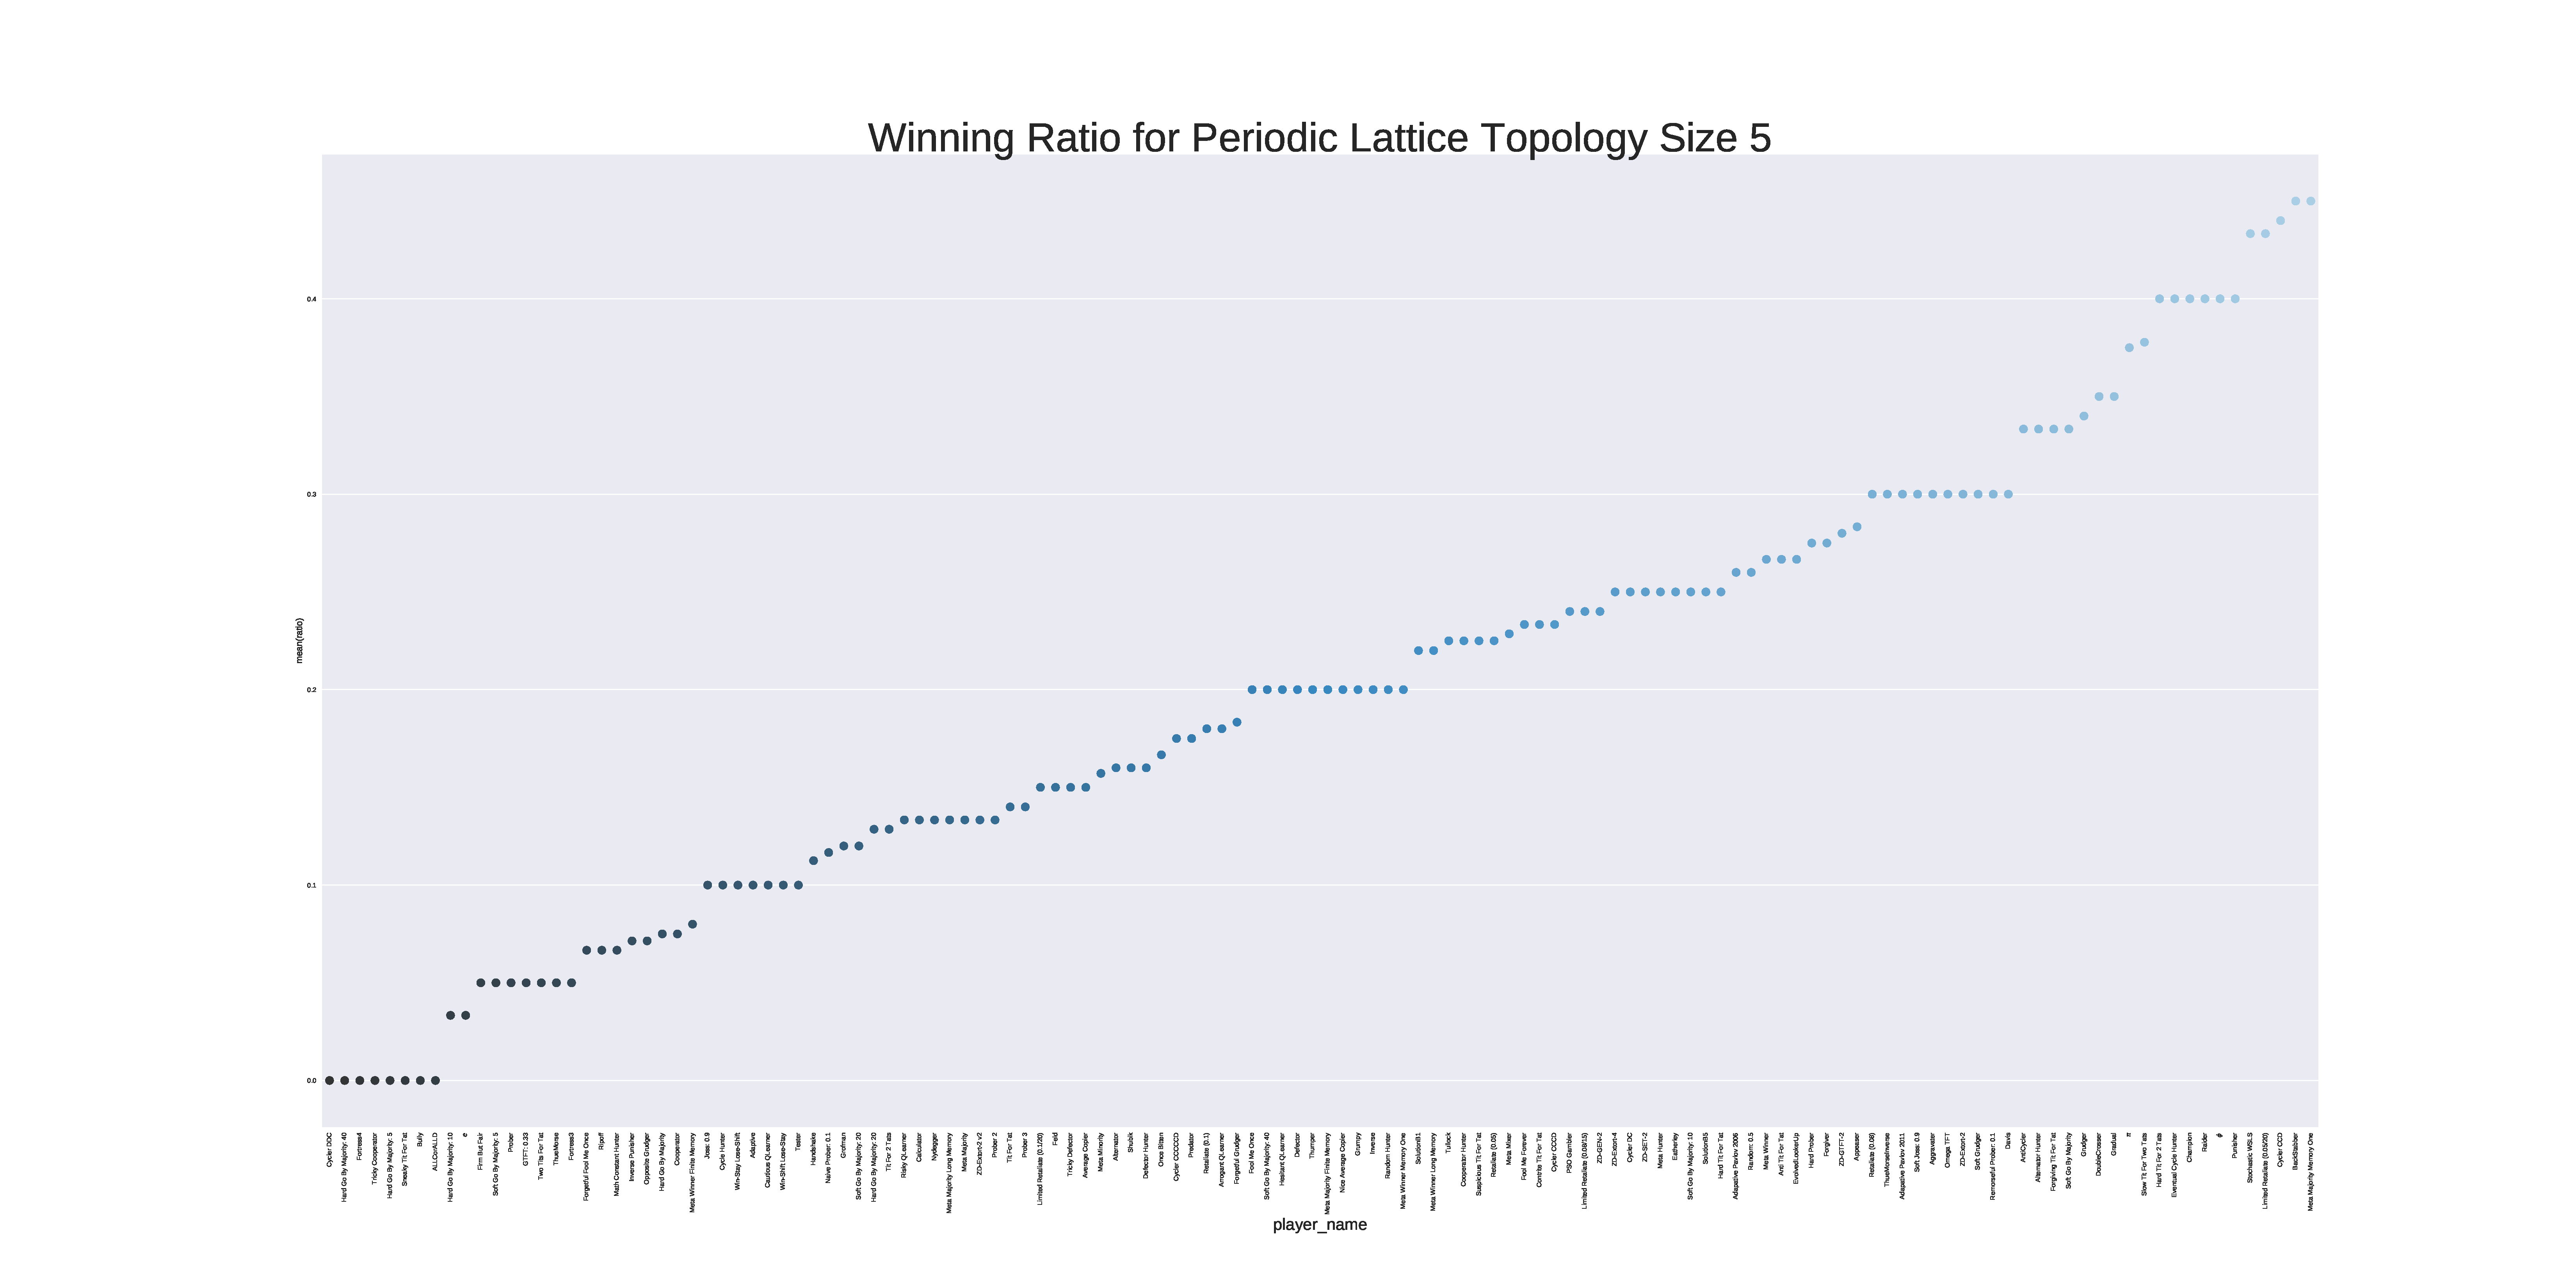
\includegraphics[width=\linewidth]{appendix/winners-Periodic-Lattice-5.pdf}
    \caption{Winning ration lattice s=5.}
    \end{subfigure}
\hfill
    \begin{subfigure}[t]{1\textwidth}\centering
    \centering
        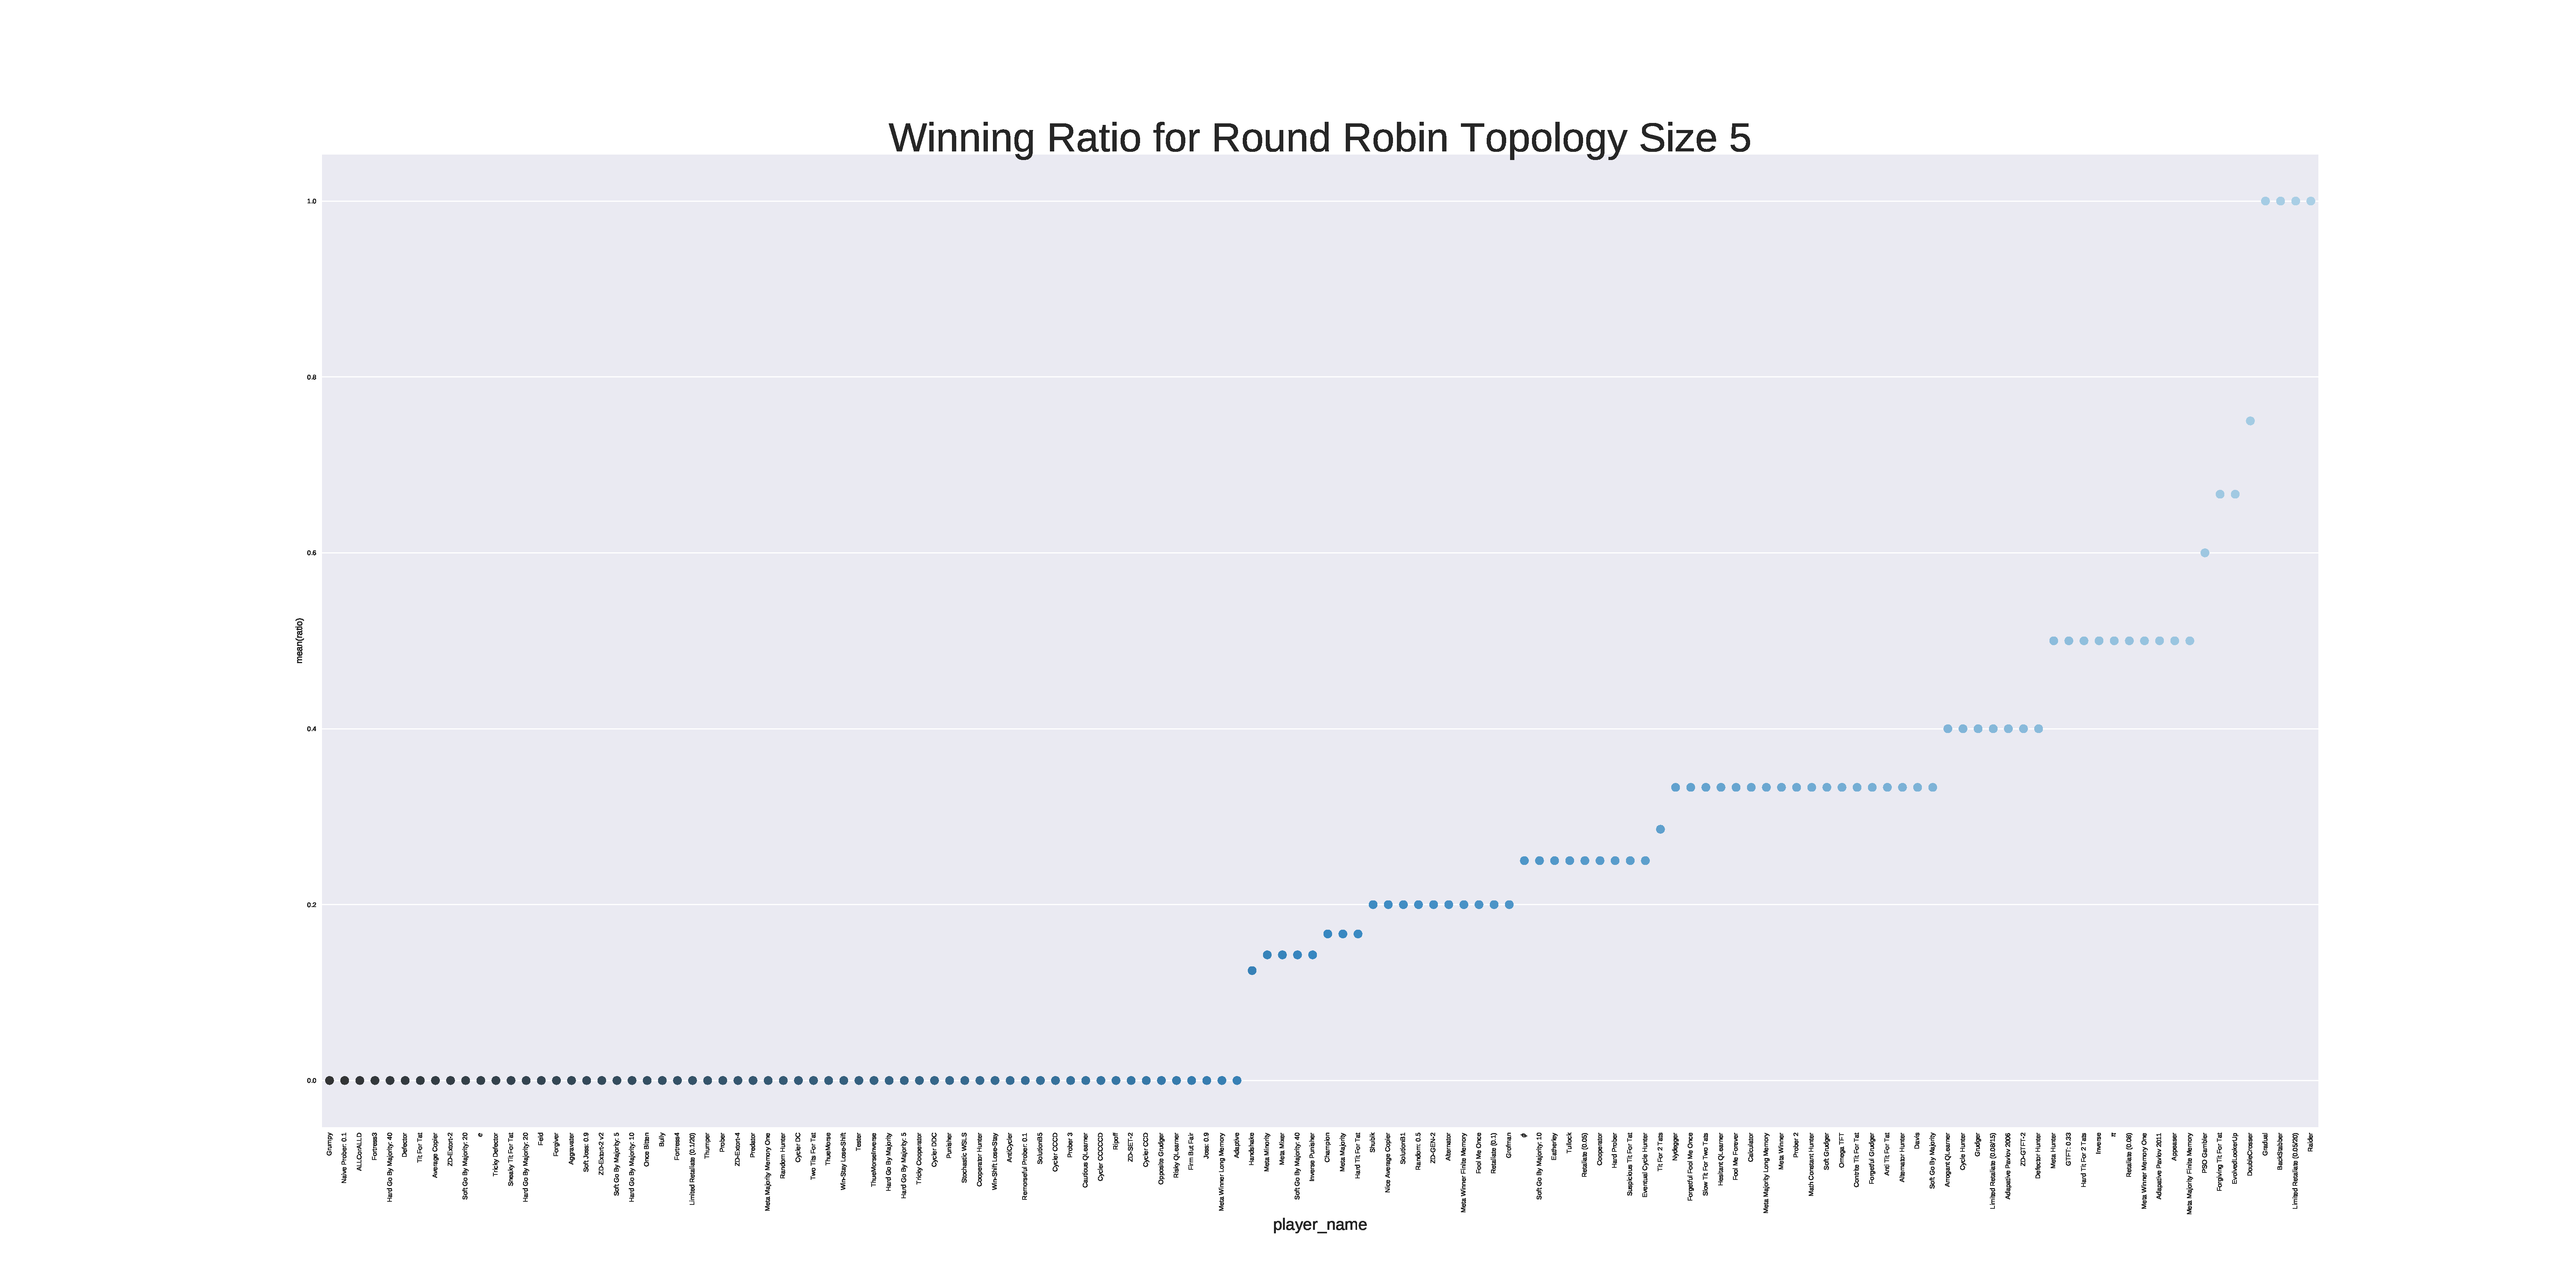
\includegraphics[width=\linewidth]{appendix/winners-Round-Robin-5.pdf}
    \caption{Winning ration round robin s=5.}
    \end{subfigure}
\caption{Winning ratio for all three topologies s=5.}
\label{fig:winning-five}

\end{figure}

\begin{figure}[H]
\centering
    \begin{subfigure}[t]{1\textwidth}
    \centering
        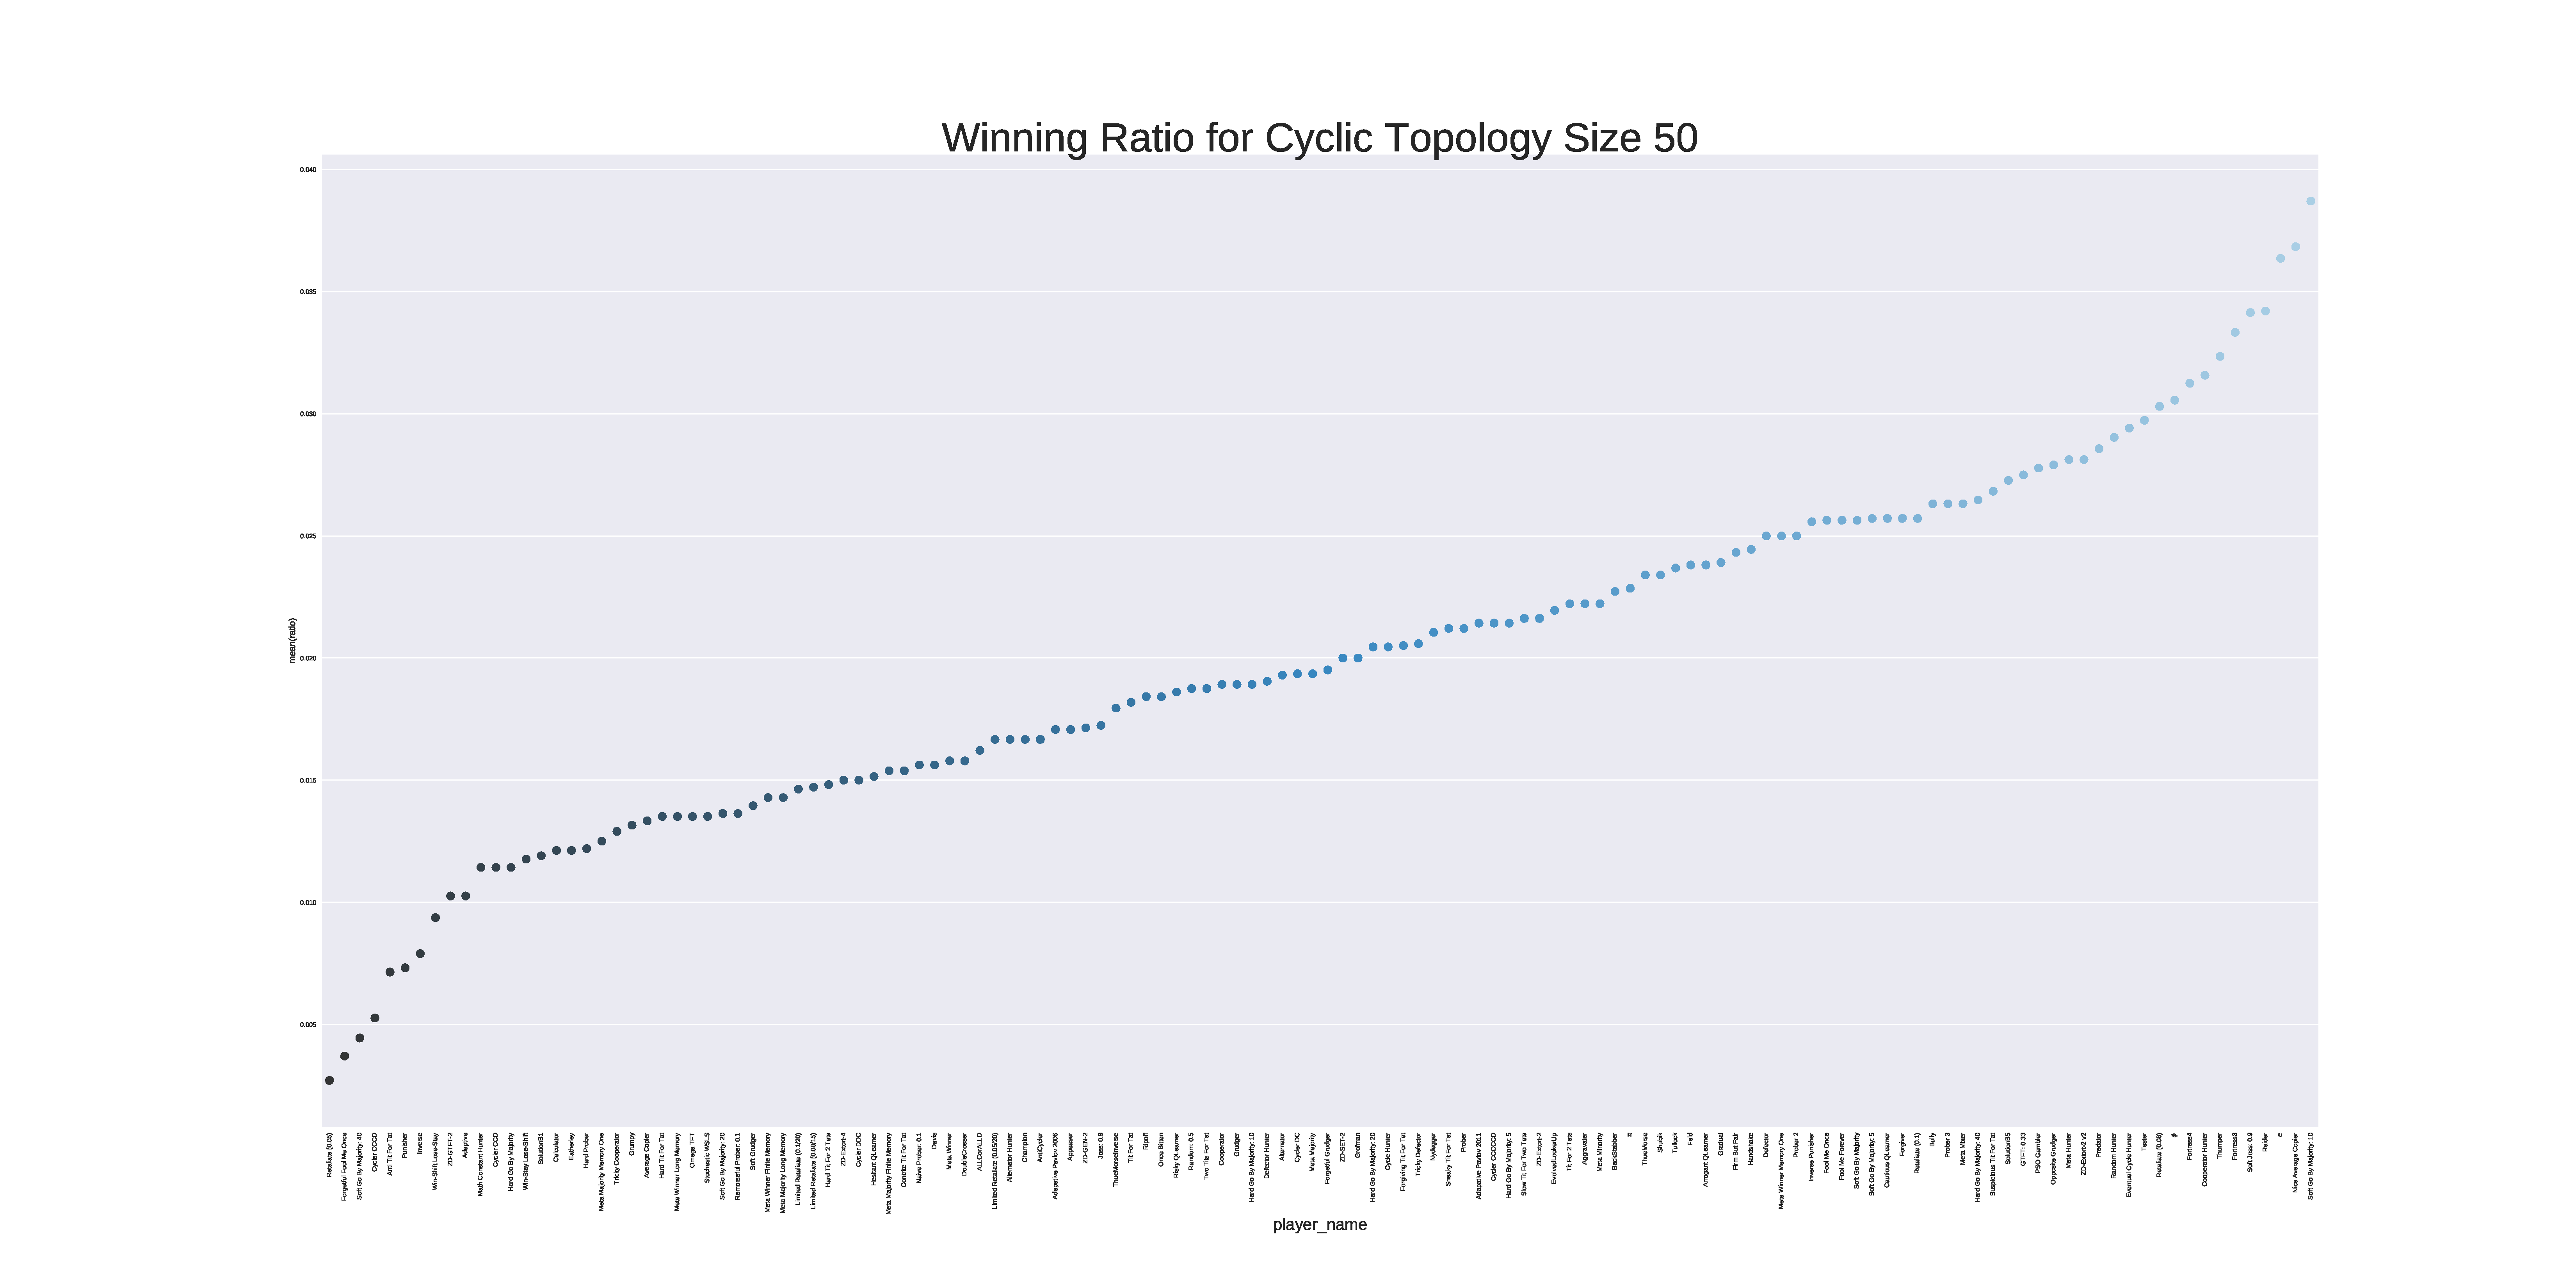
\includegraphics[width=\linewidth]{appendix/winners-Cyclic-50.pdf}
    \caption{Winning ration cyclic s=50.}
    \end{subfigure}
\hfill
    \begin{subfigure}[t]{1\textwidth}\centering
    \centering
        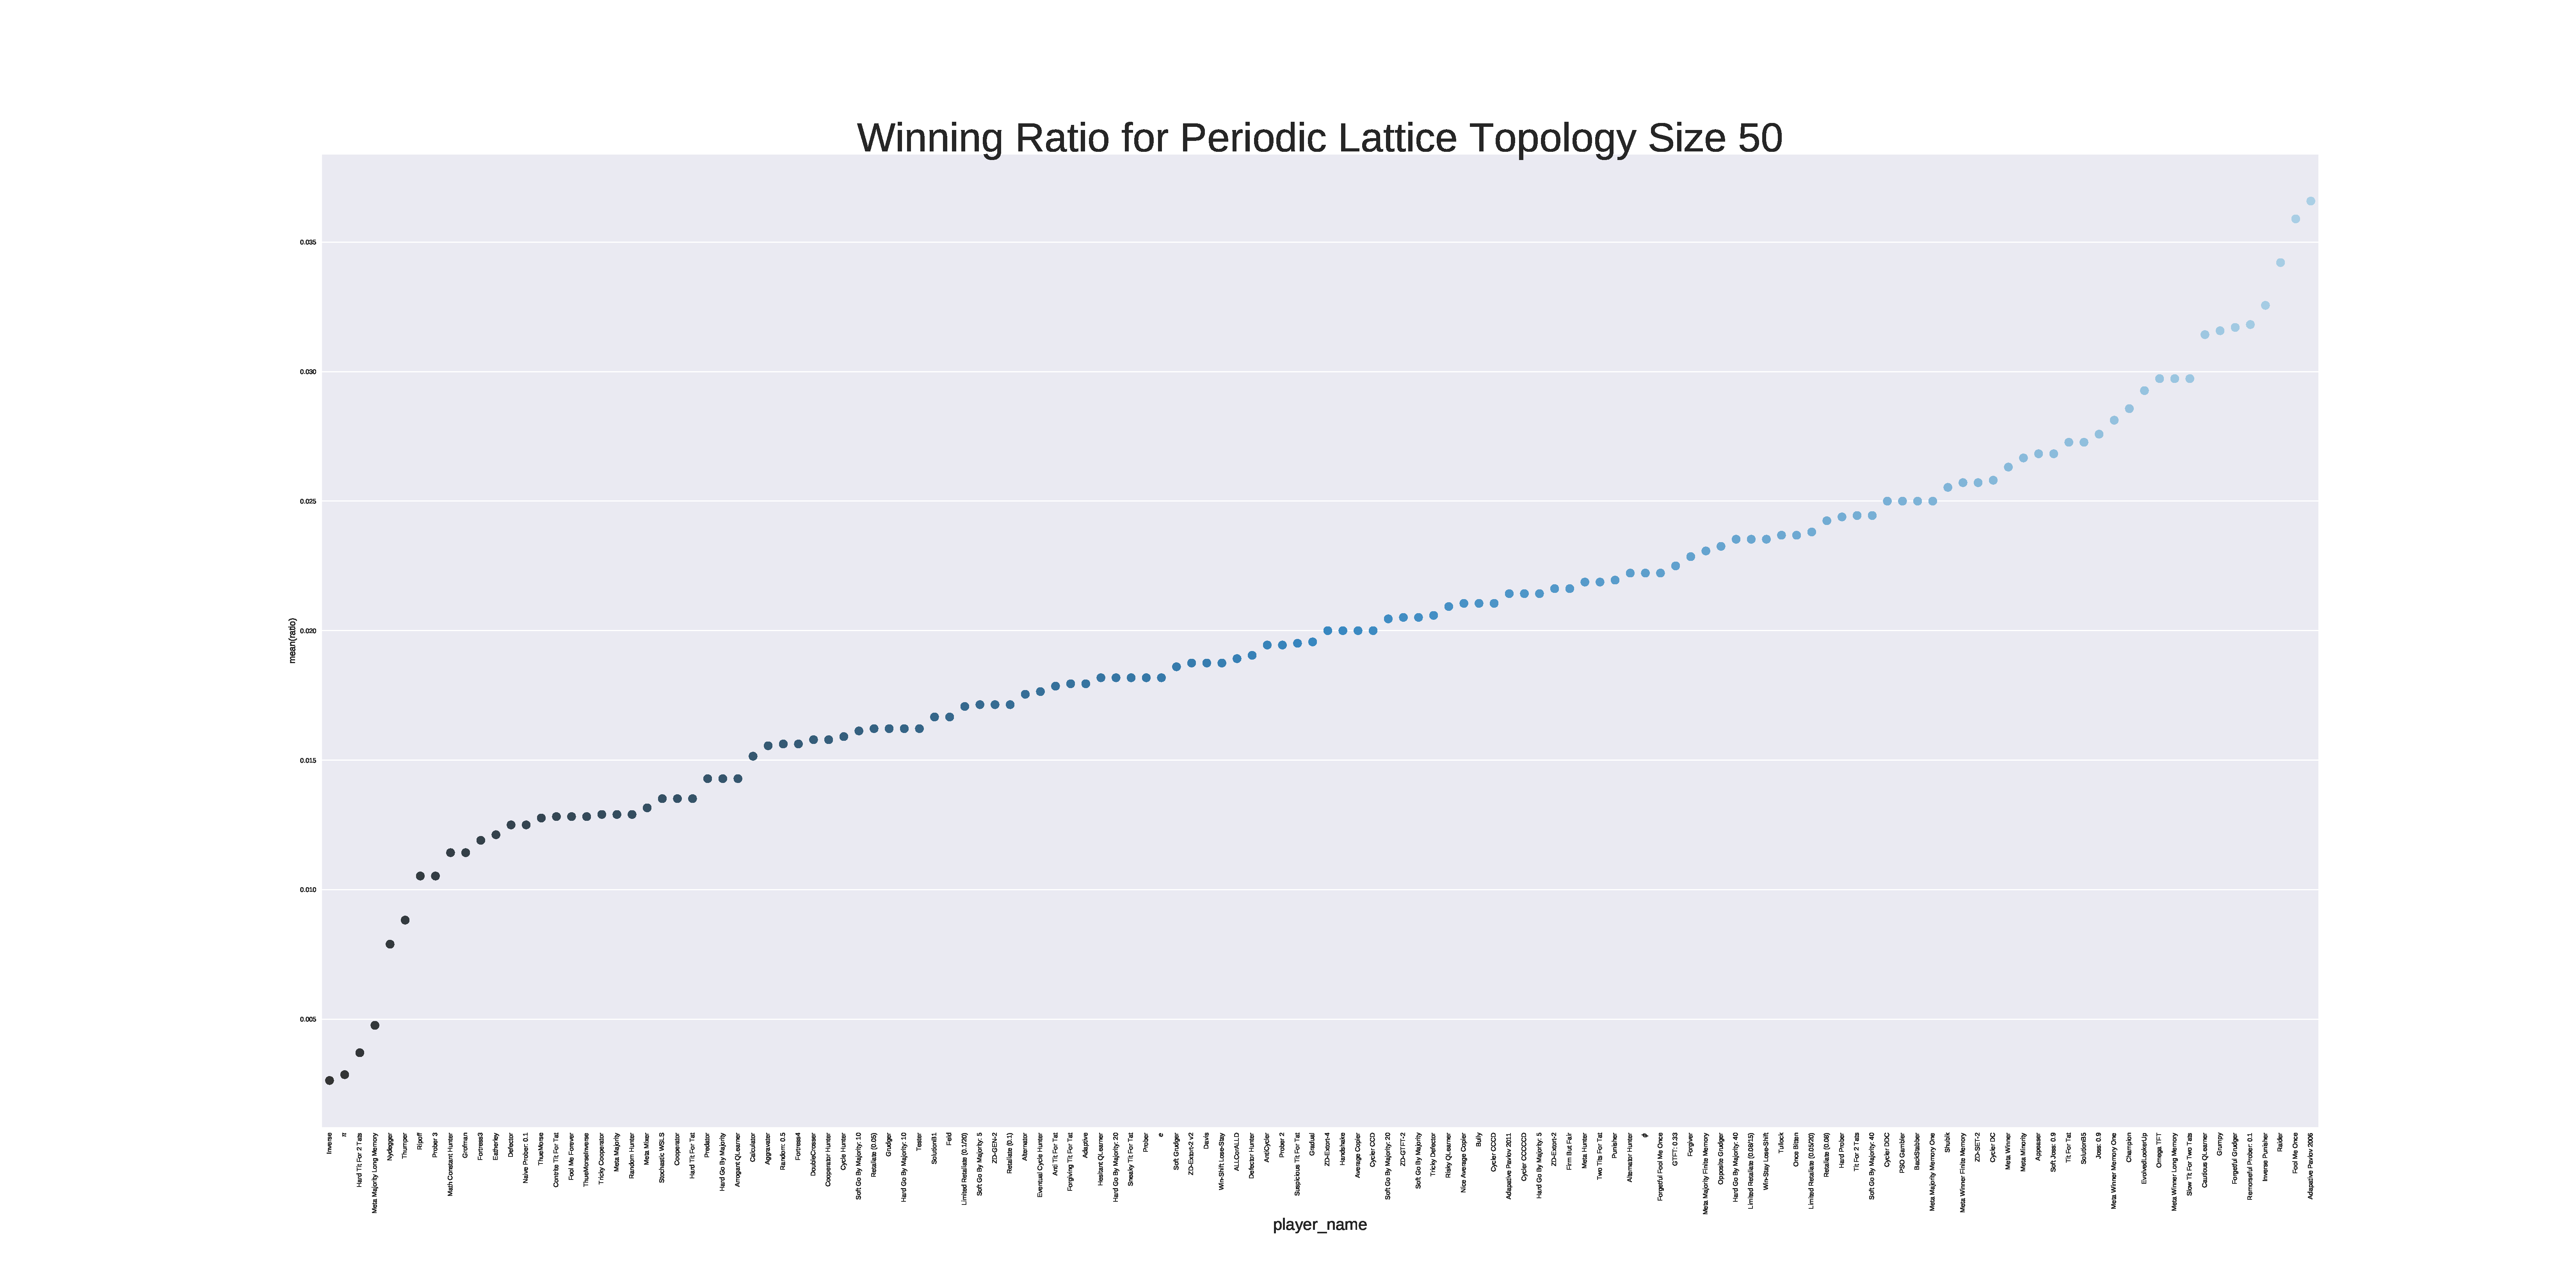
\includegraphics[width=\linewidth]{appendix/winners-Periodic-Lattice-50.pdf}
    \caption{Winning ration lattice s=50.}
    \end{subfigure}
\hfill
    \begin{subfigure}[t]{1\textwidth}\centering
    \centering
        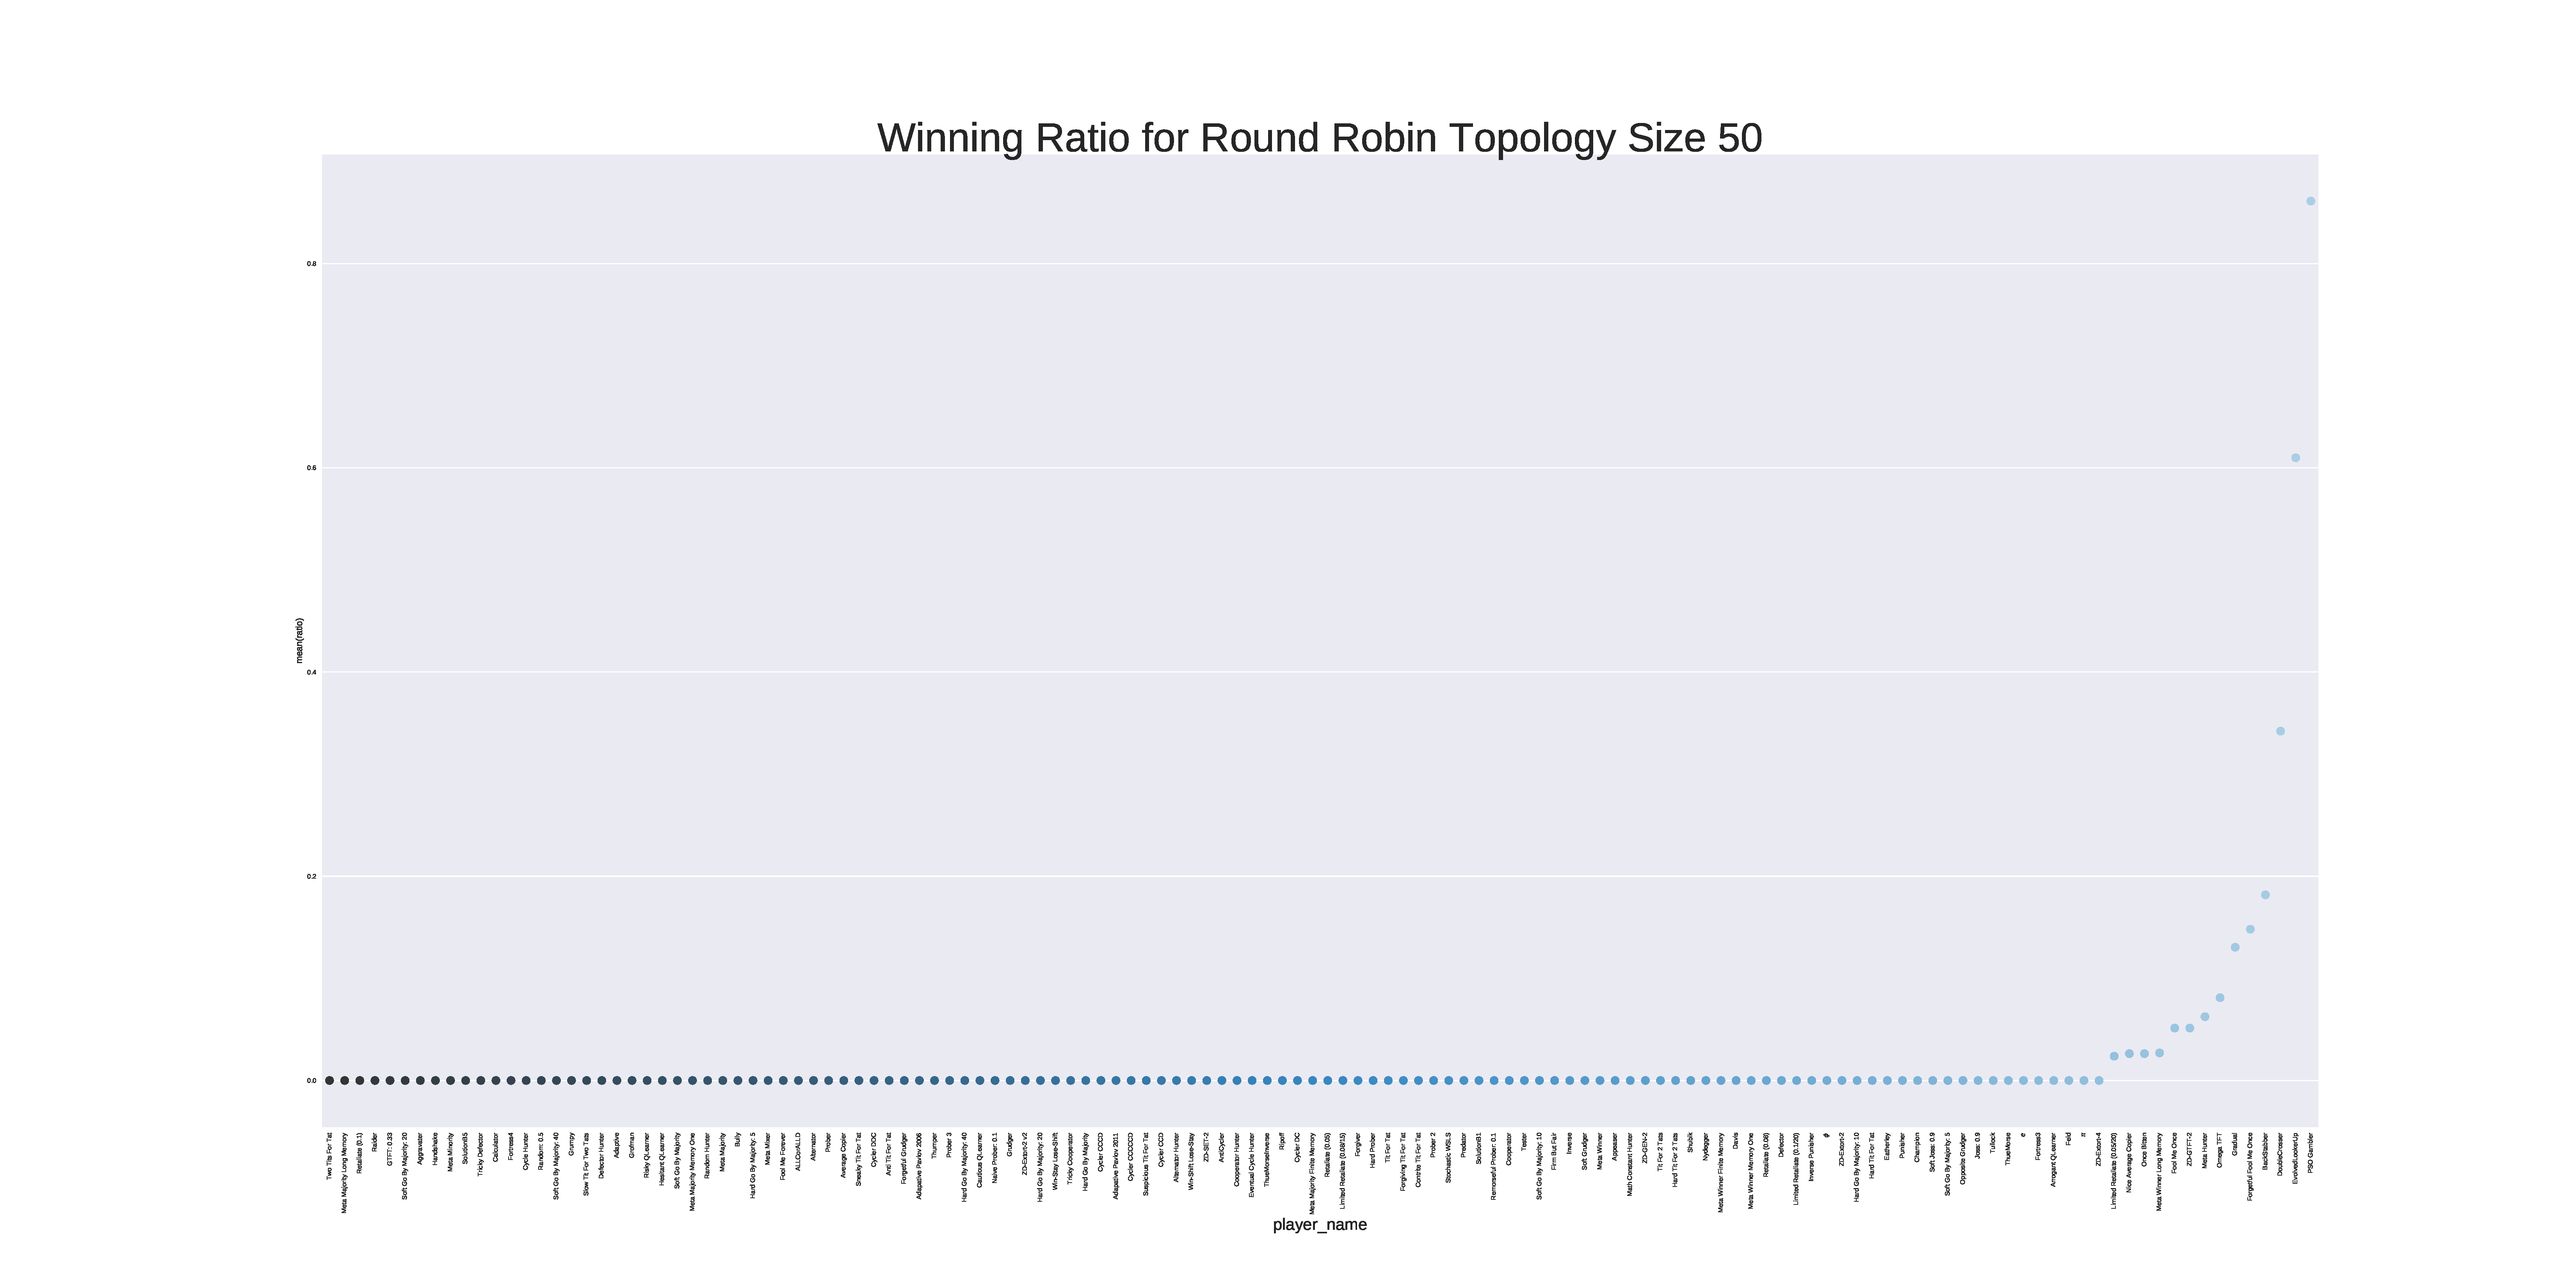
\includegraphics[width=\linewidth]{appendix/winners-Round-Robin-50.pdf}
    \caption{Winning ration round robin s=50.}
    \end{subfigure}
\caption{Winning ratio for all three topologies s=50.}
\label{fig:winning-fifty}
\end{figure}

\subsection{Variation plots for normalized average score, simple networks}
\label{append:variation-plots}
In this section, as explained in~\ref{chap:Three}, the variation of the
normalized average score has been plotted. These plots are found here.

\begin{figure}[h]
\centering
    \begin{subfigure}[t]{0.8\textwidth}
    \centering
        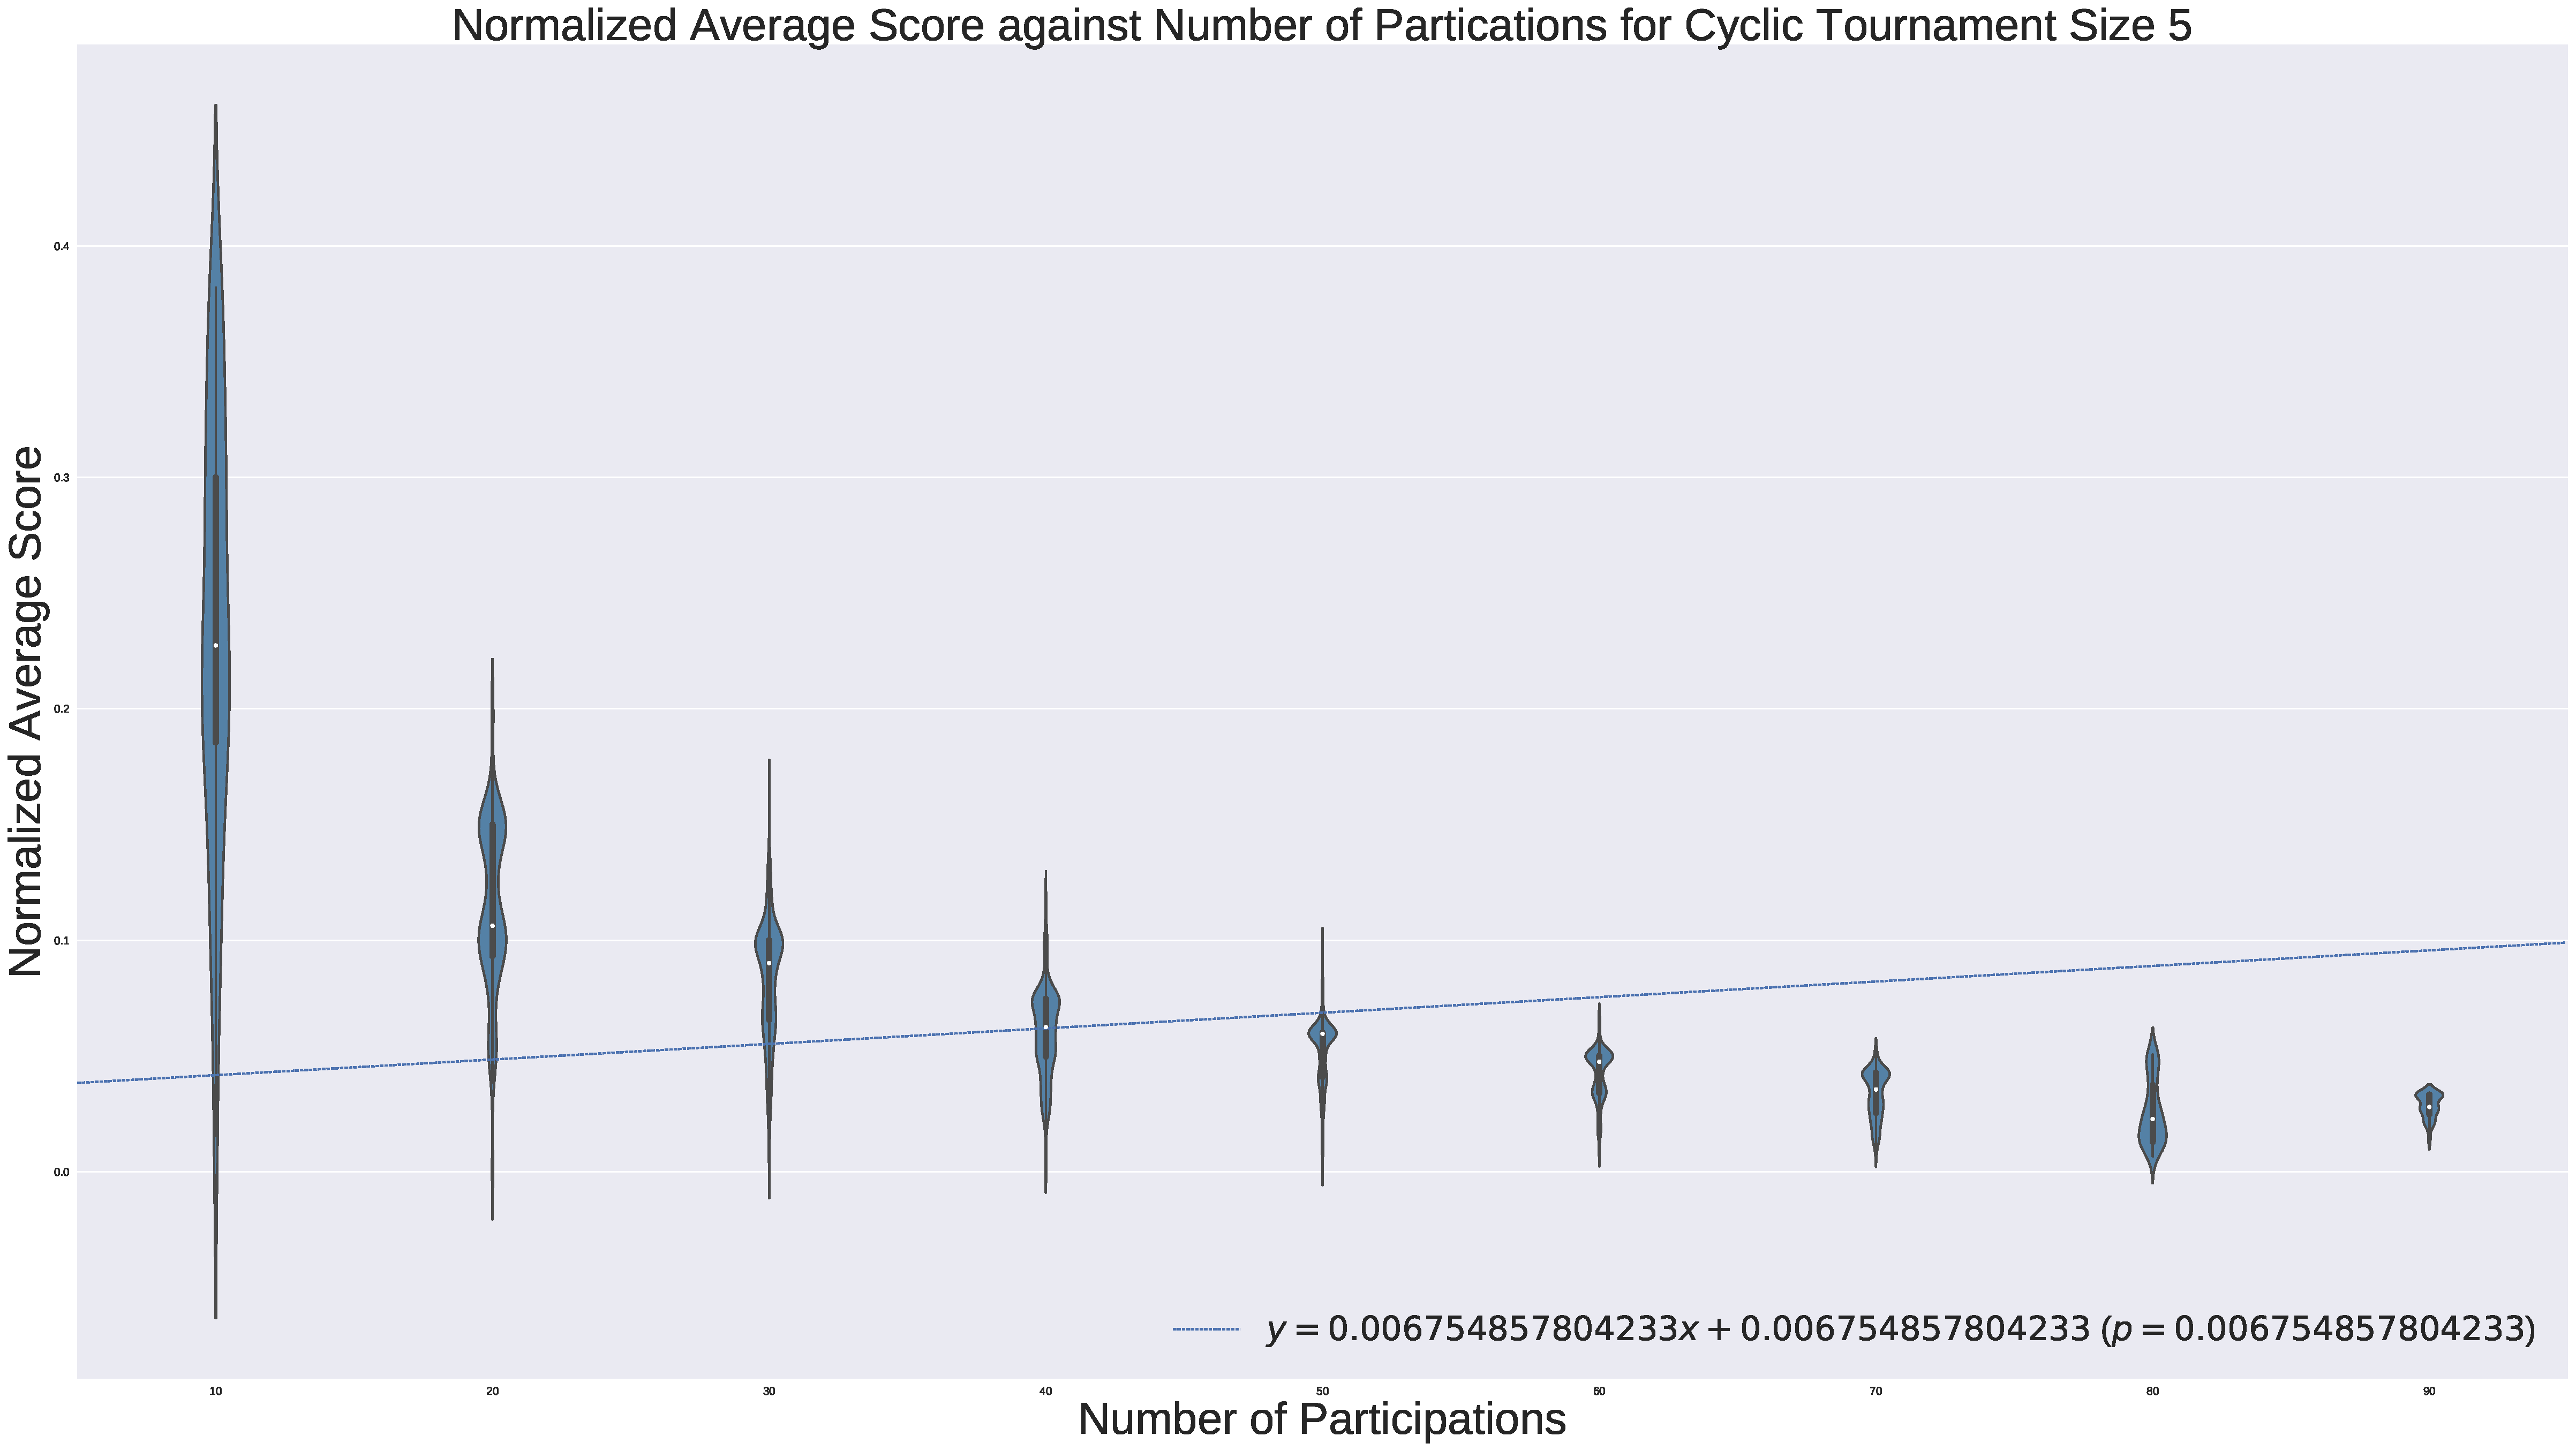
\includegraphics[width=\linewidth]{chapter-three/normalized-score-Cyclic-5.pdf}
    \caption{Normalized Average Score Cyclic Topology Size 5.}
    \end{subfigure}
\hfill
    \begin{subfigure}[t]{0.8\textwidth}\centering
    \centering
        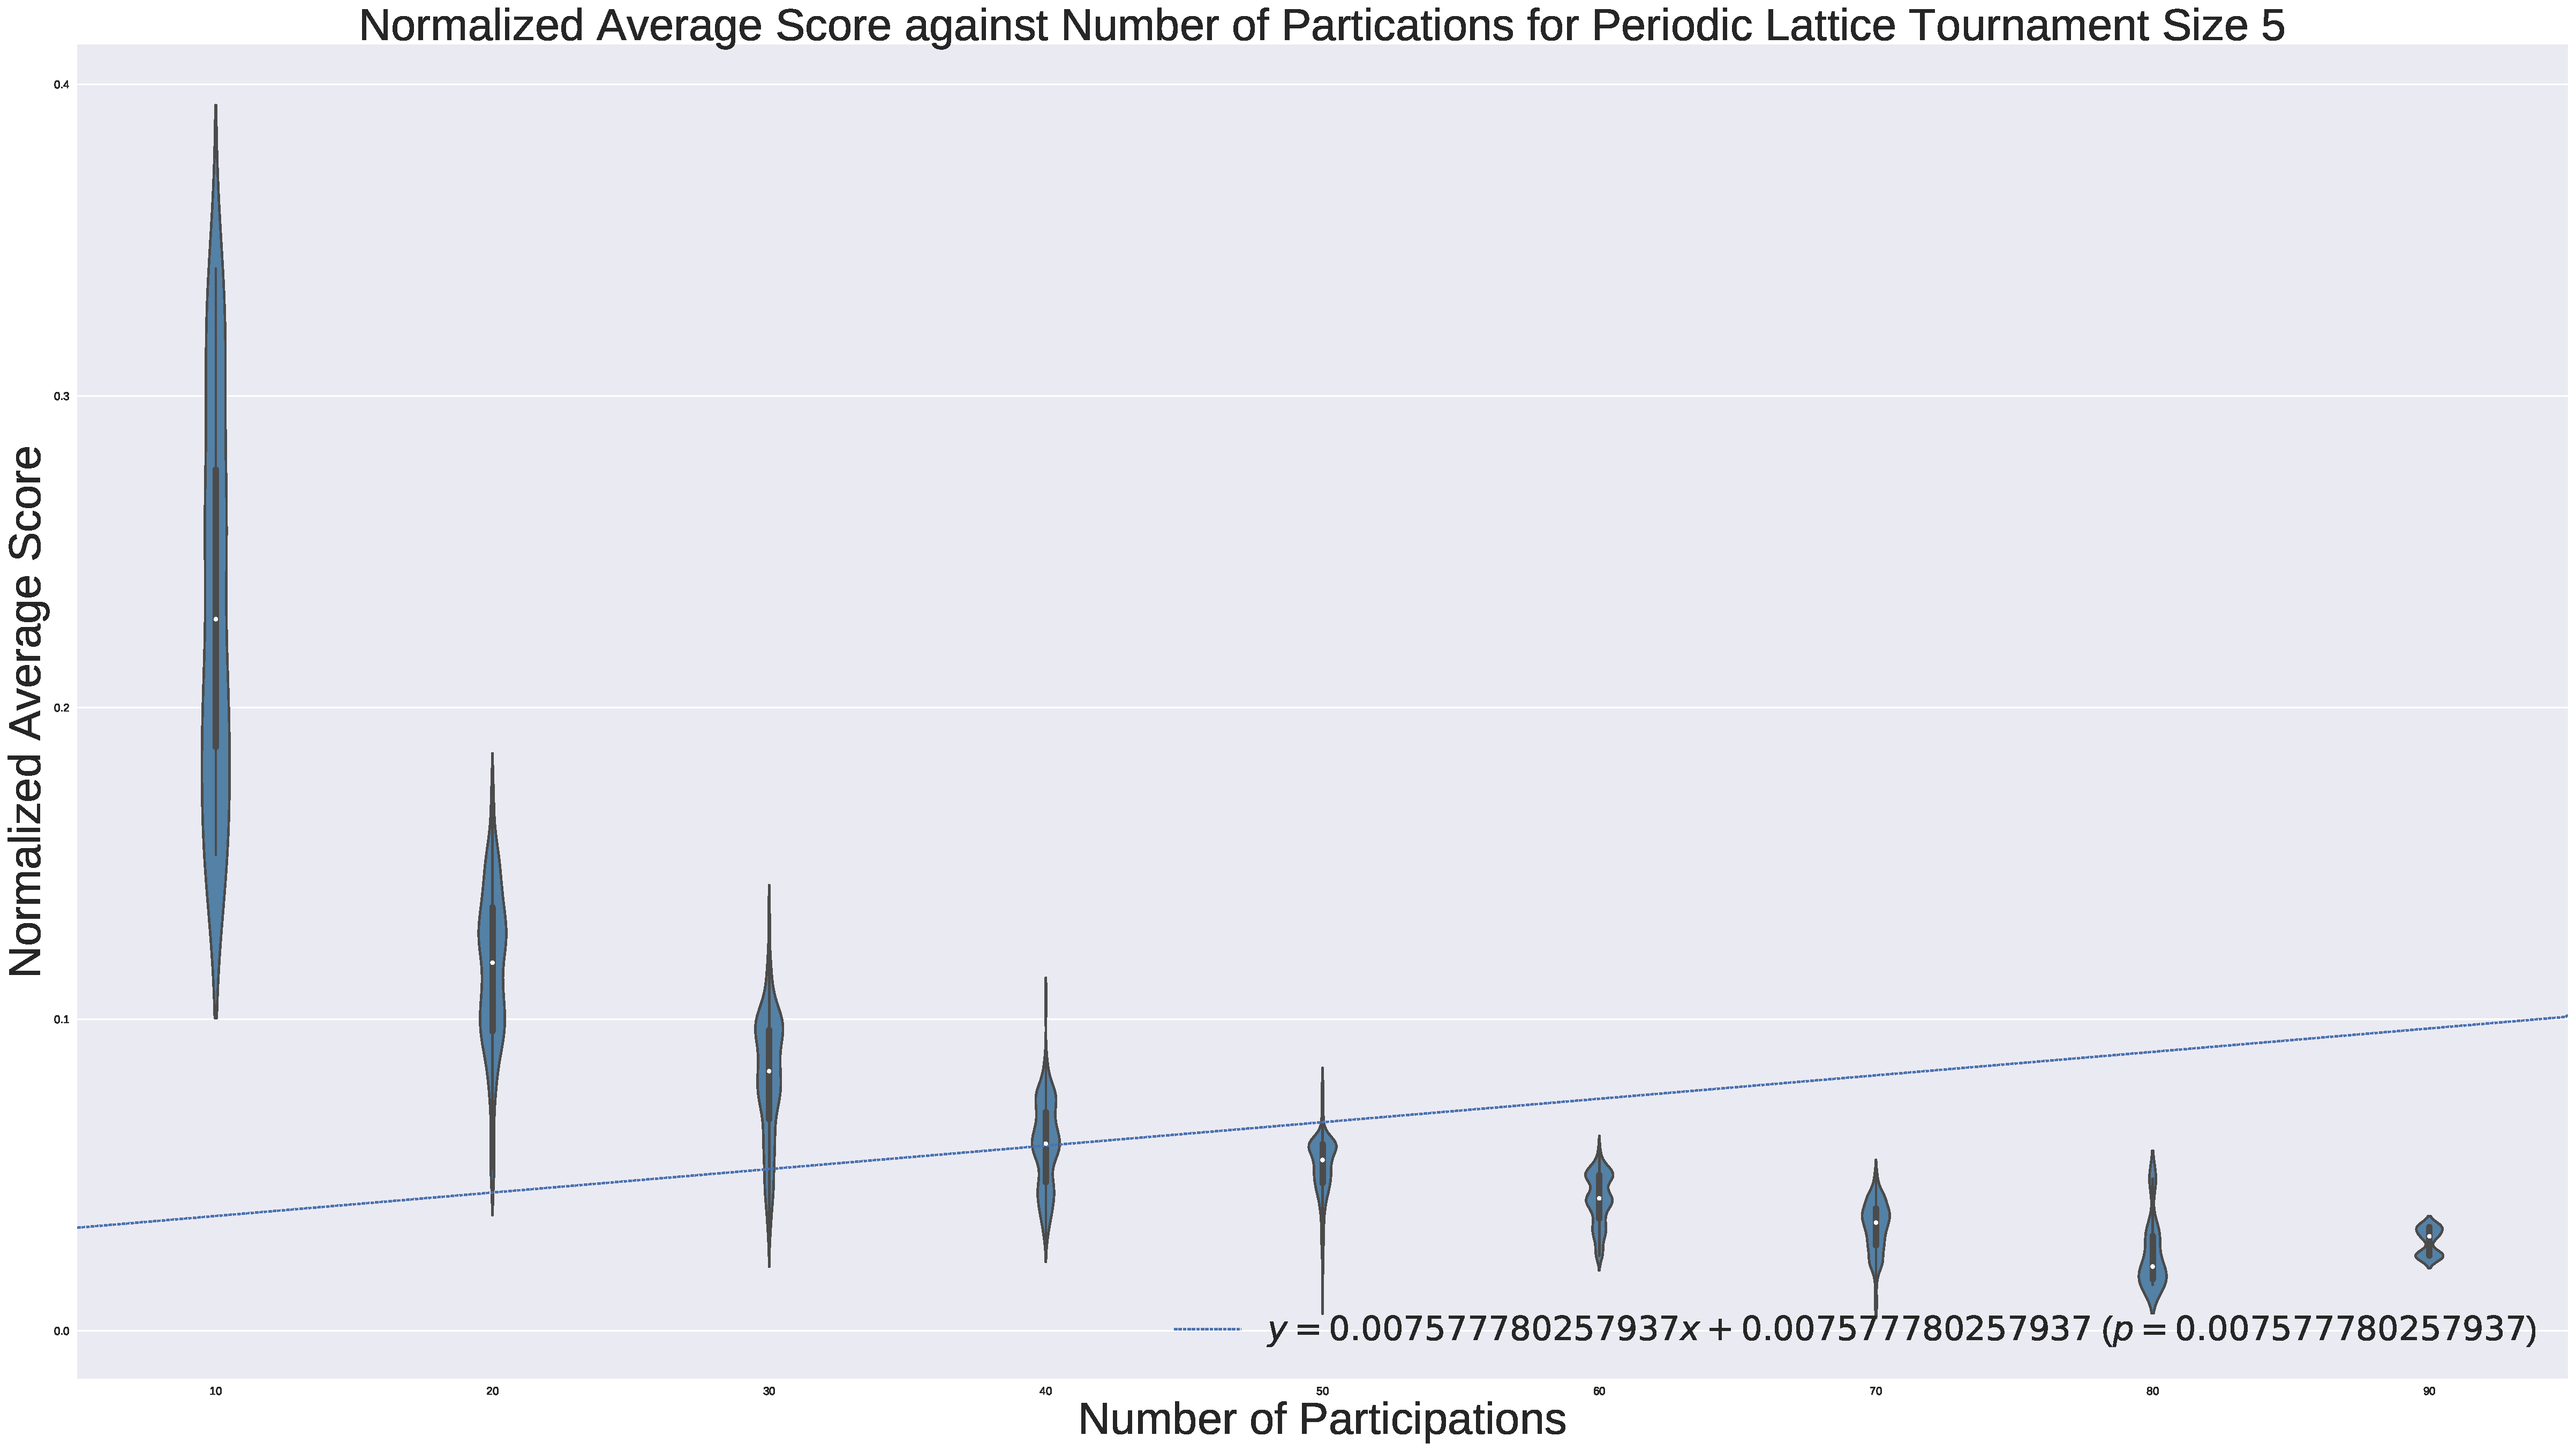
\includegraphics[width=\linewidth]{chapter-three/normalized-score-Periodic-Lattice-5.pdf}
    \caption{Normalized Average Score Periodic Lattice Topology Size 5.}
    \end{subfigure}
\hfill
    \begin{subfigure}[t]{0.8\textwidth}\centering
    \centering
        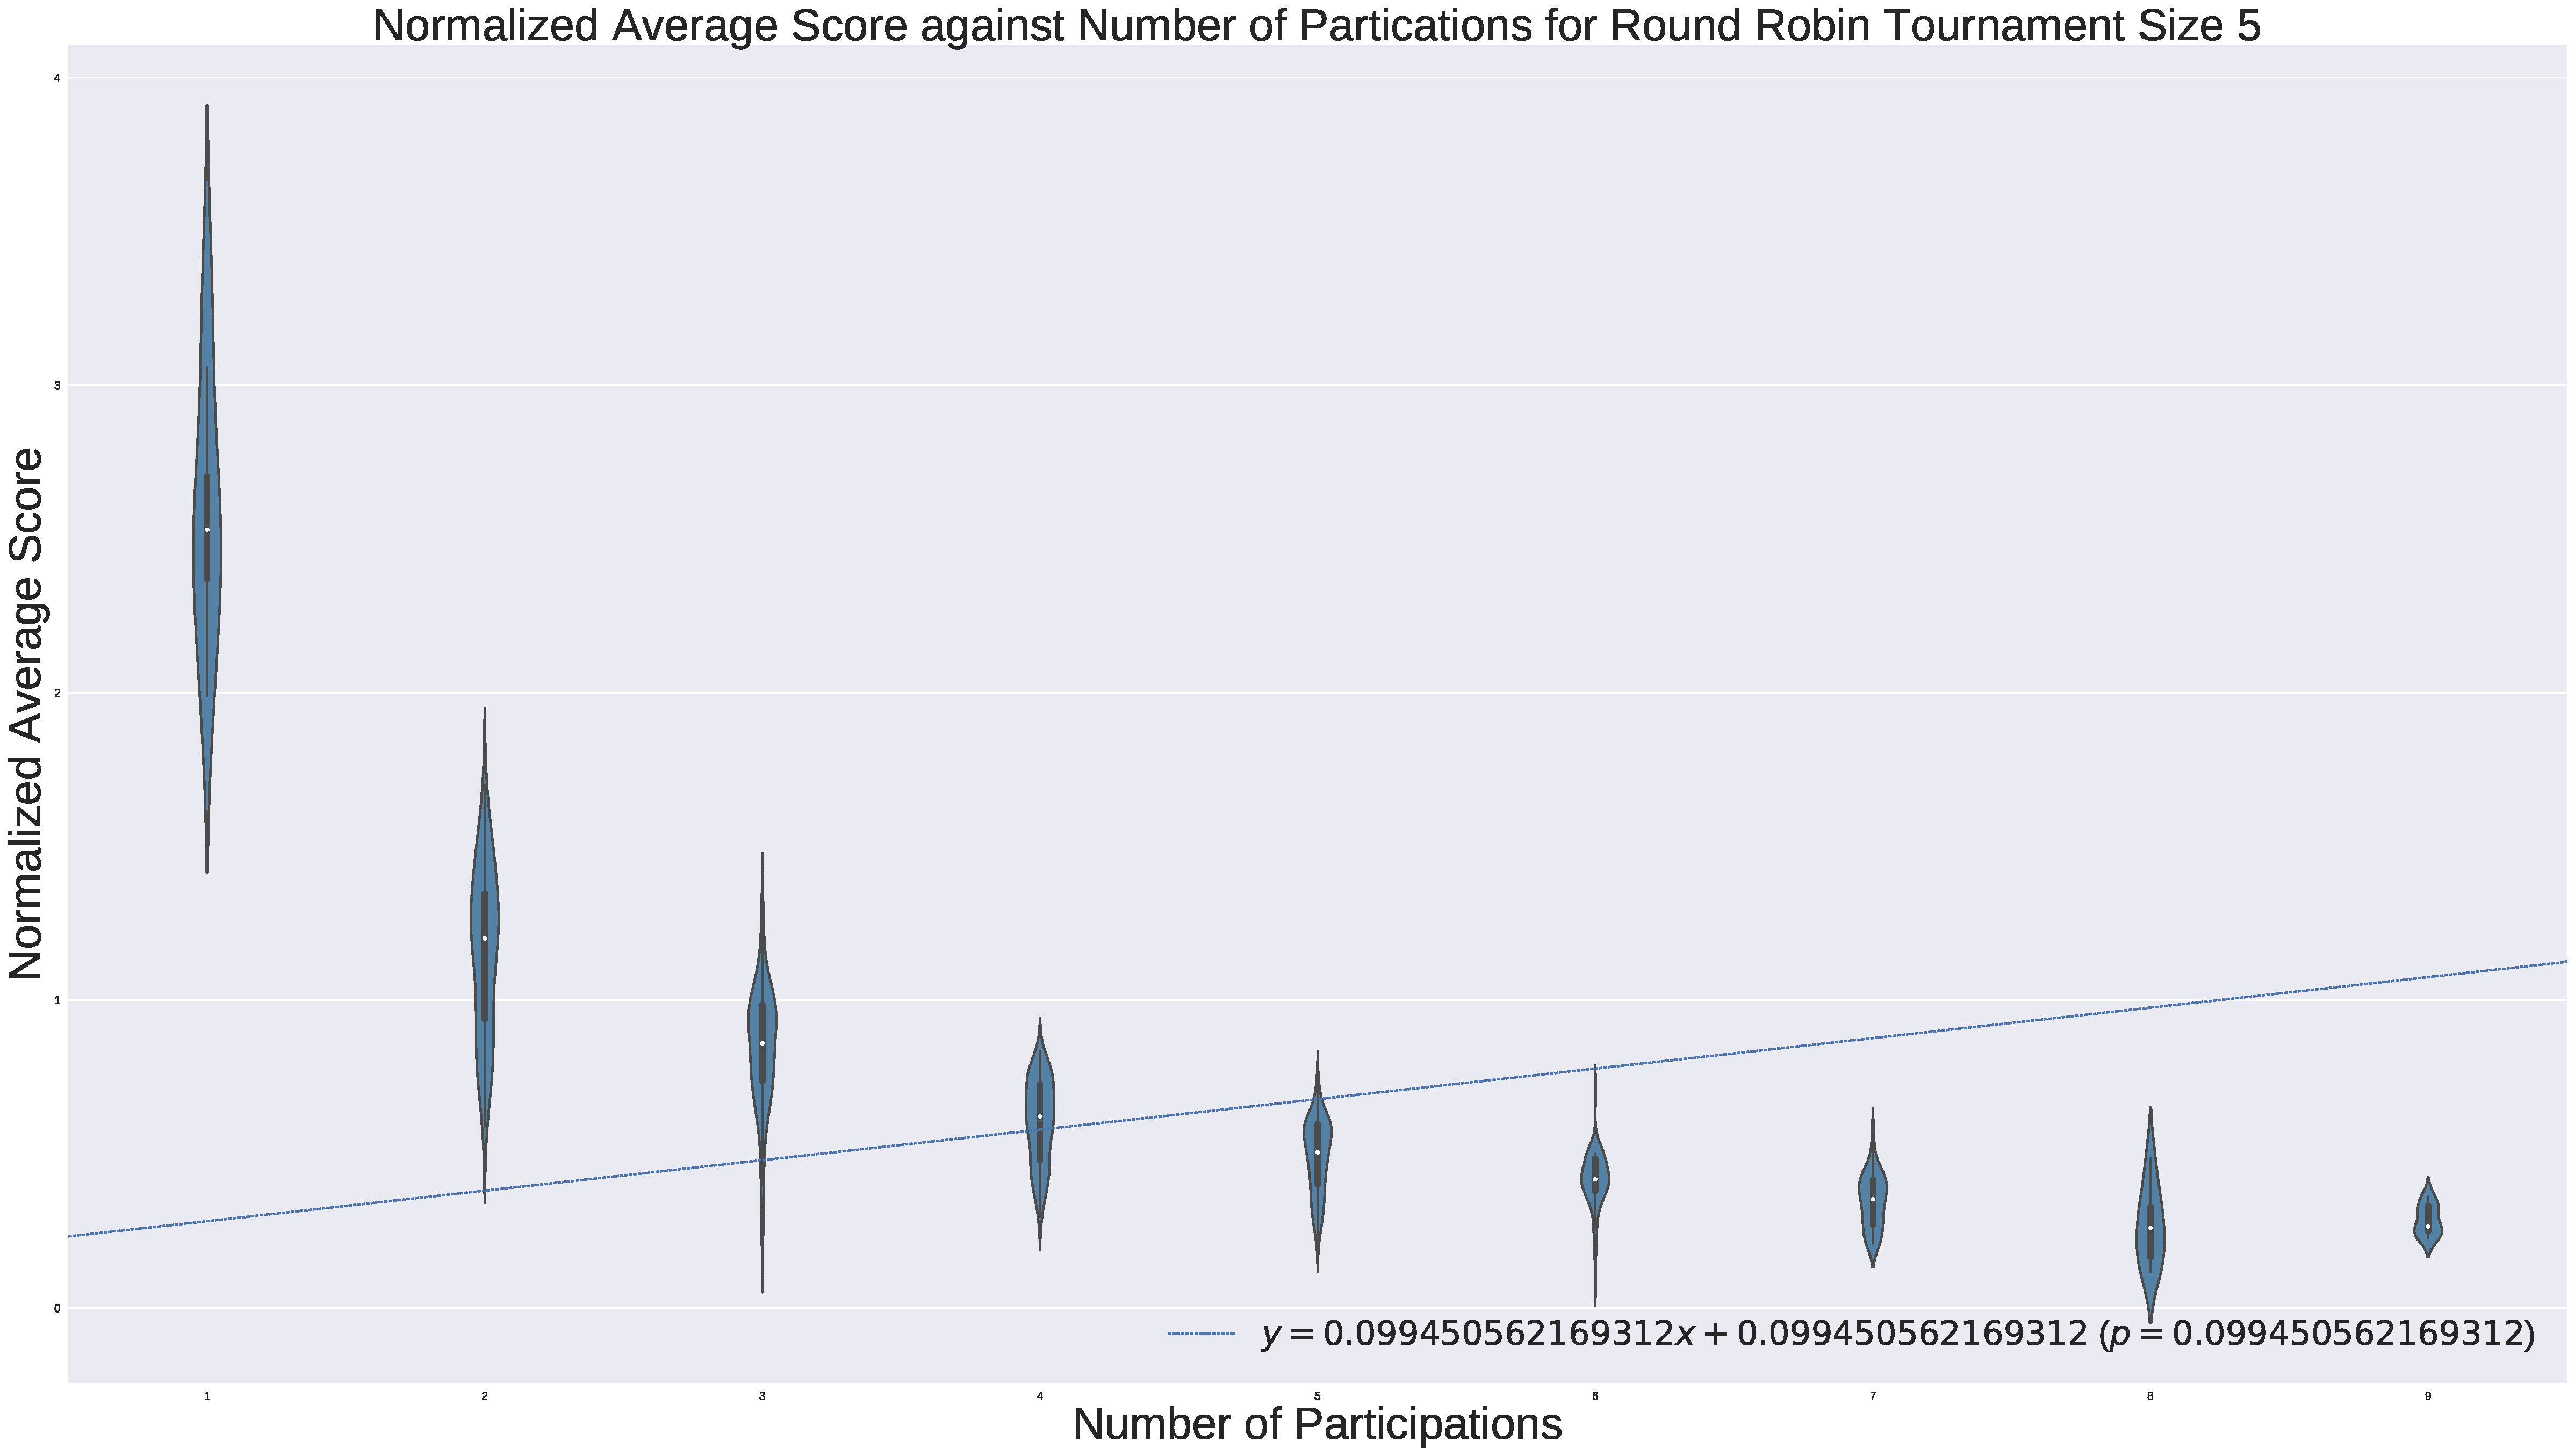
\includegraphics[width=\linewidth]{chapter-three/normalized-score-Round-Robin-5.pdf}
    \caption{Normalized Average Score Round Robin Topology Size 5.}
    \end{subfigure}
\caption{Normalized Average Score for all Three Topologies Size 5.}
\label{fig:average-score-five}
\end{figure}

\begin{figure}[h]
\centering
    \begin{subfigure}[t]{1\textwidth}
    \centering
        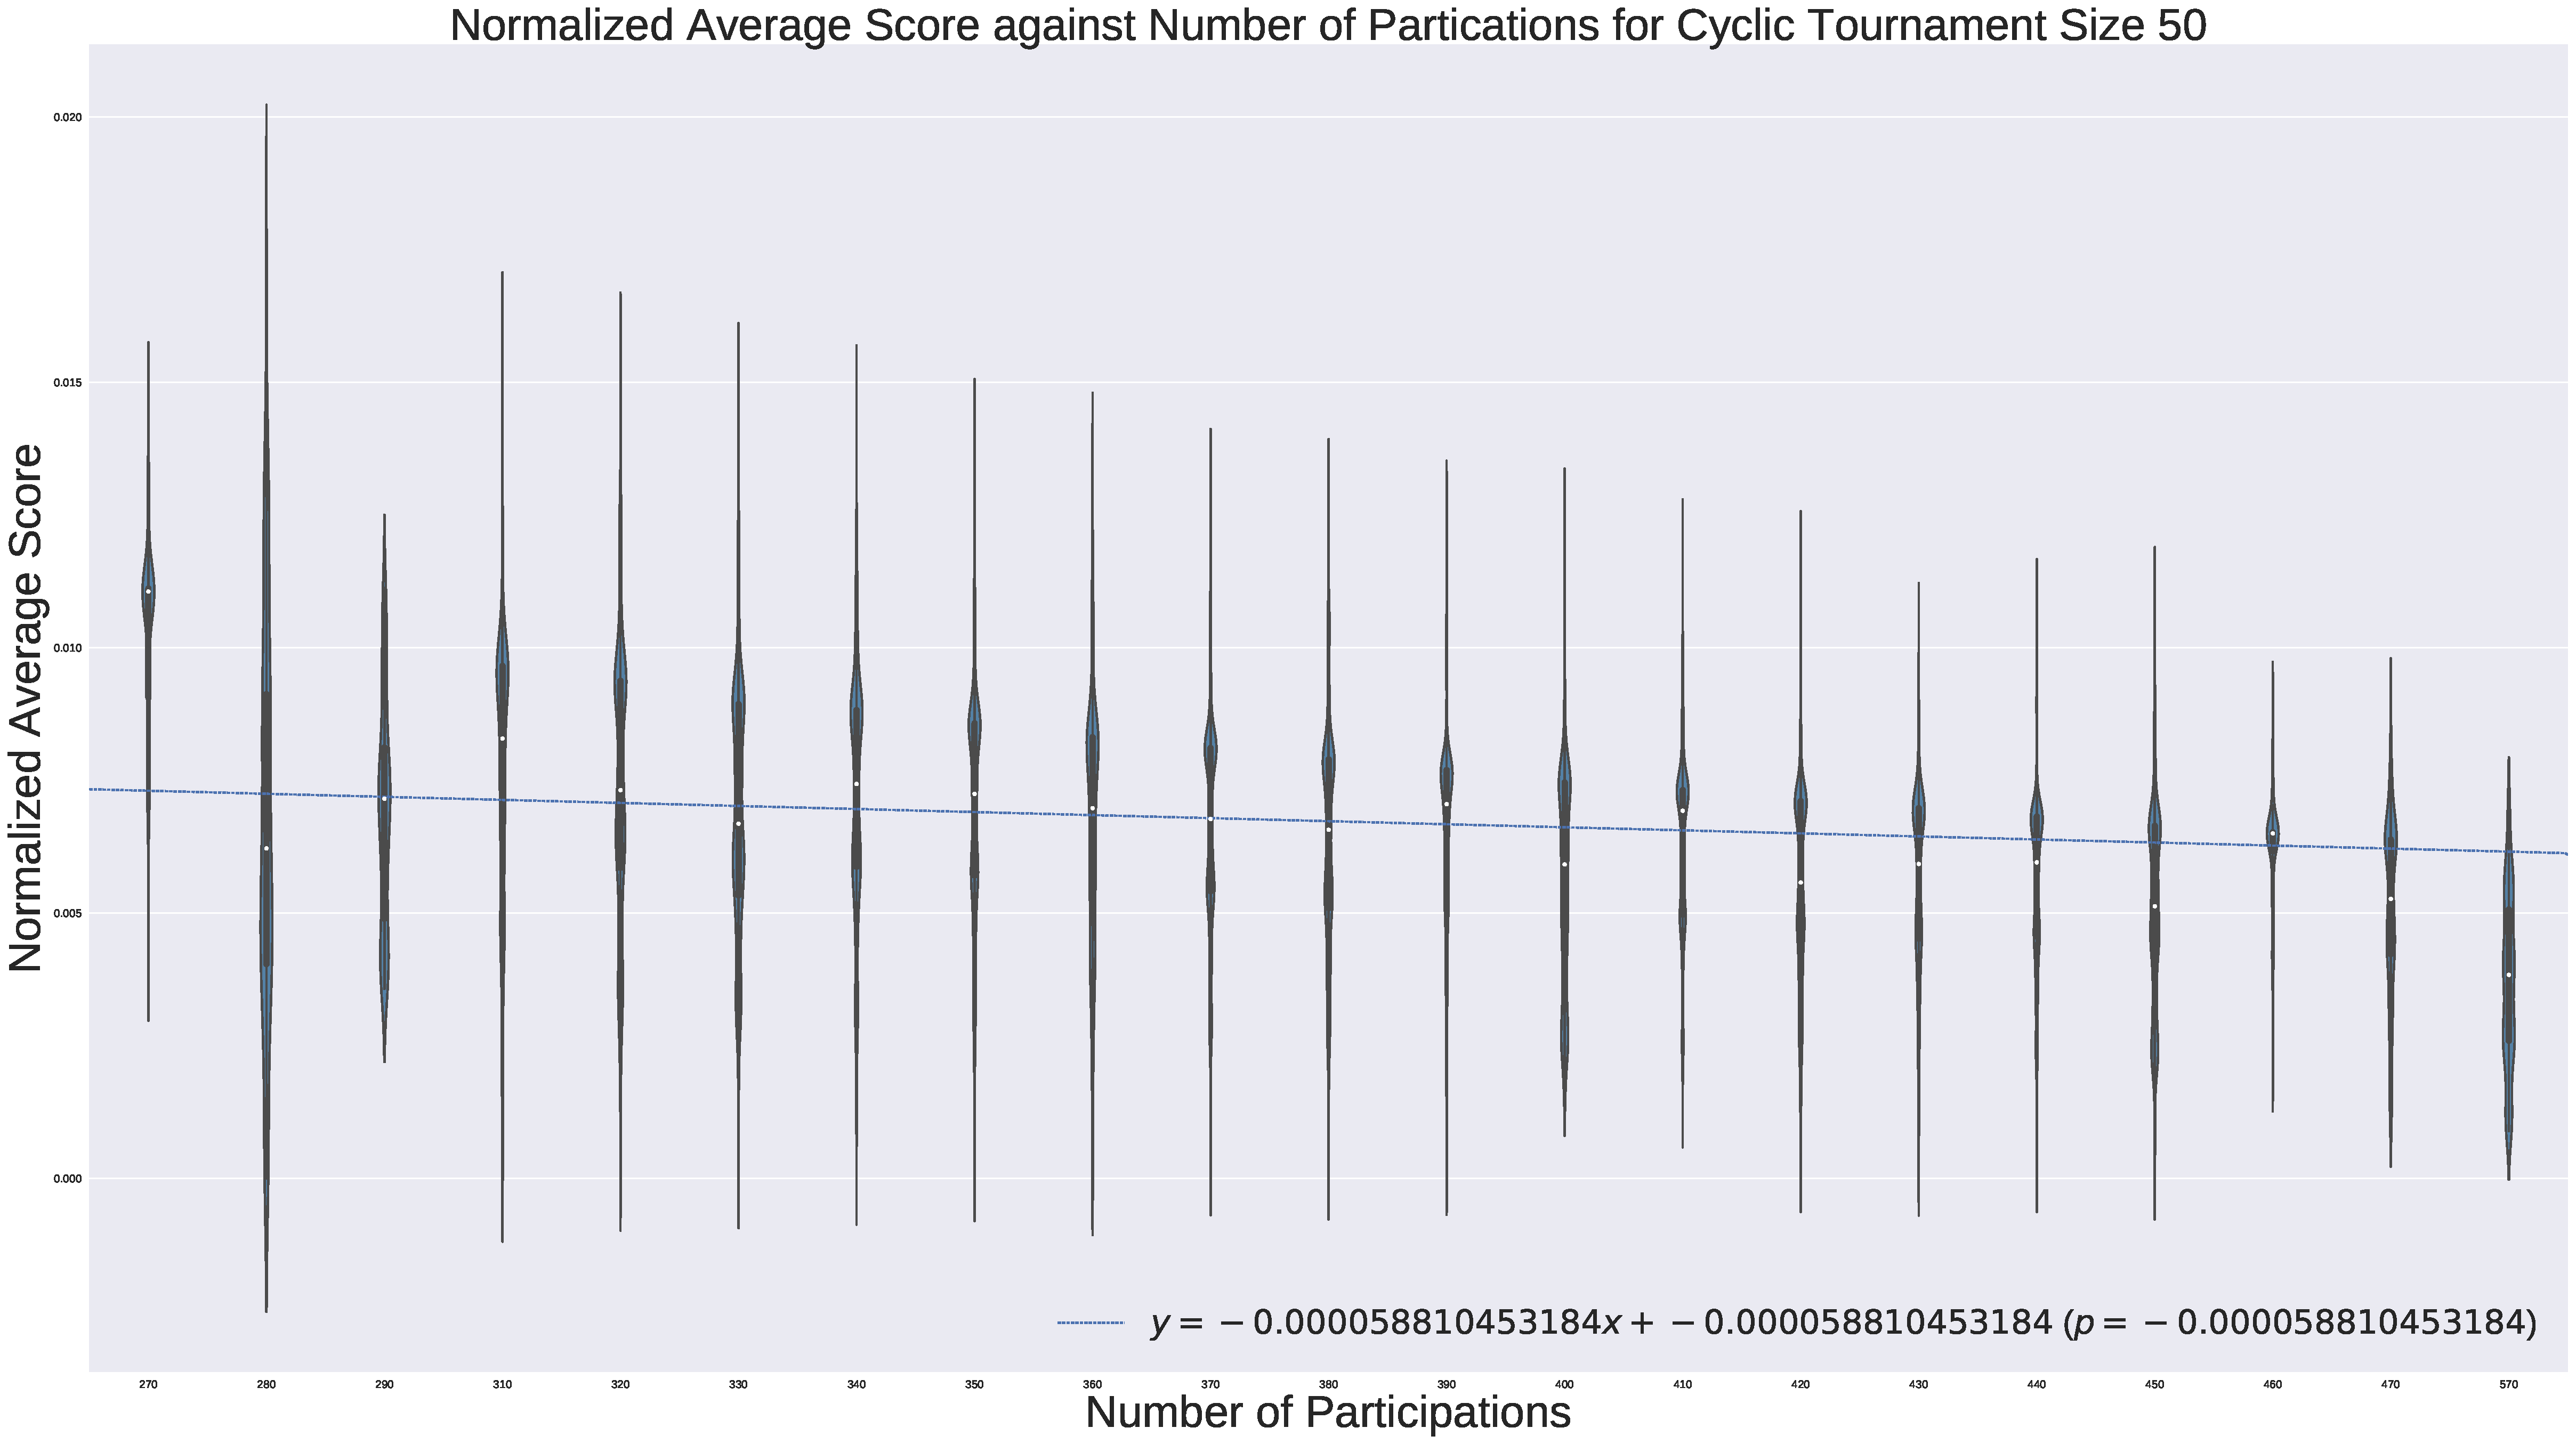
\includegraphics[width=\linewidth]{chapter-three/normalized-score-Cyclic-50.pdf}
    \caption{Normalized average score cycle s=50.}
    \end{subfigure}
\hfill
    \begin{subfigure}[t]{1\textwidth}\centering
    \centering
        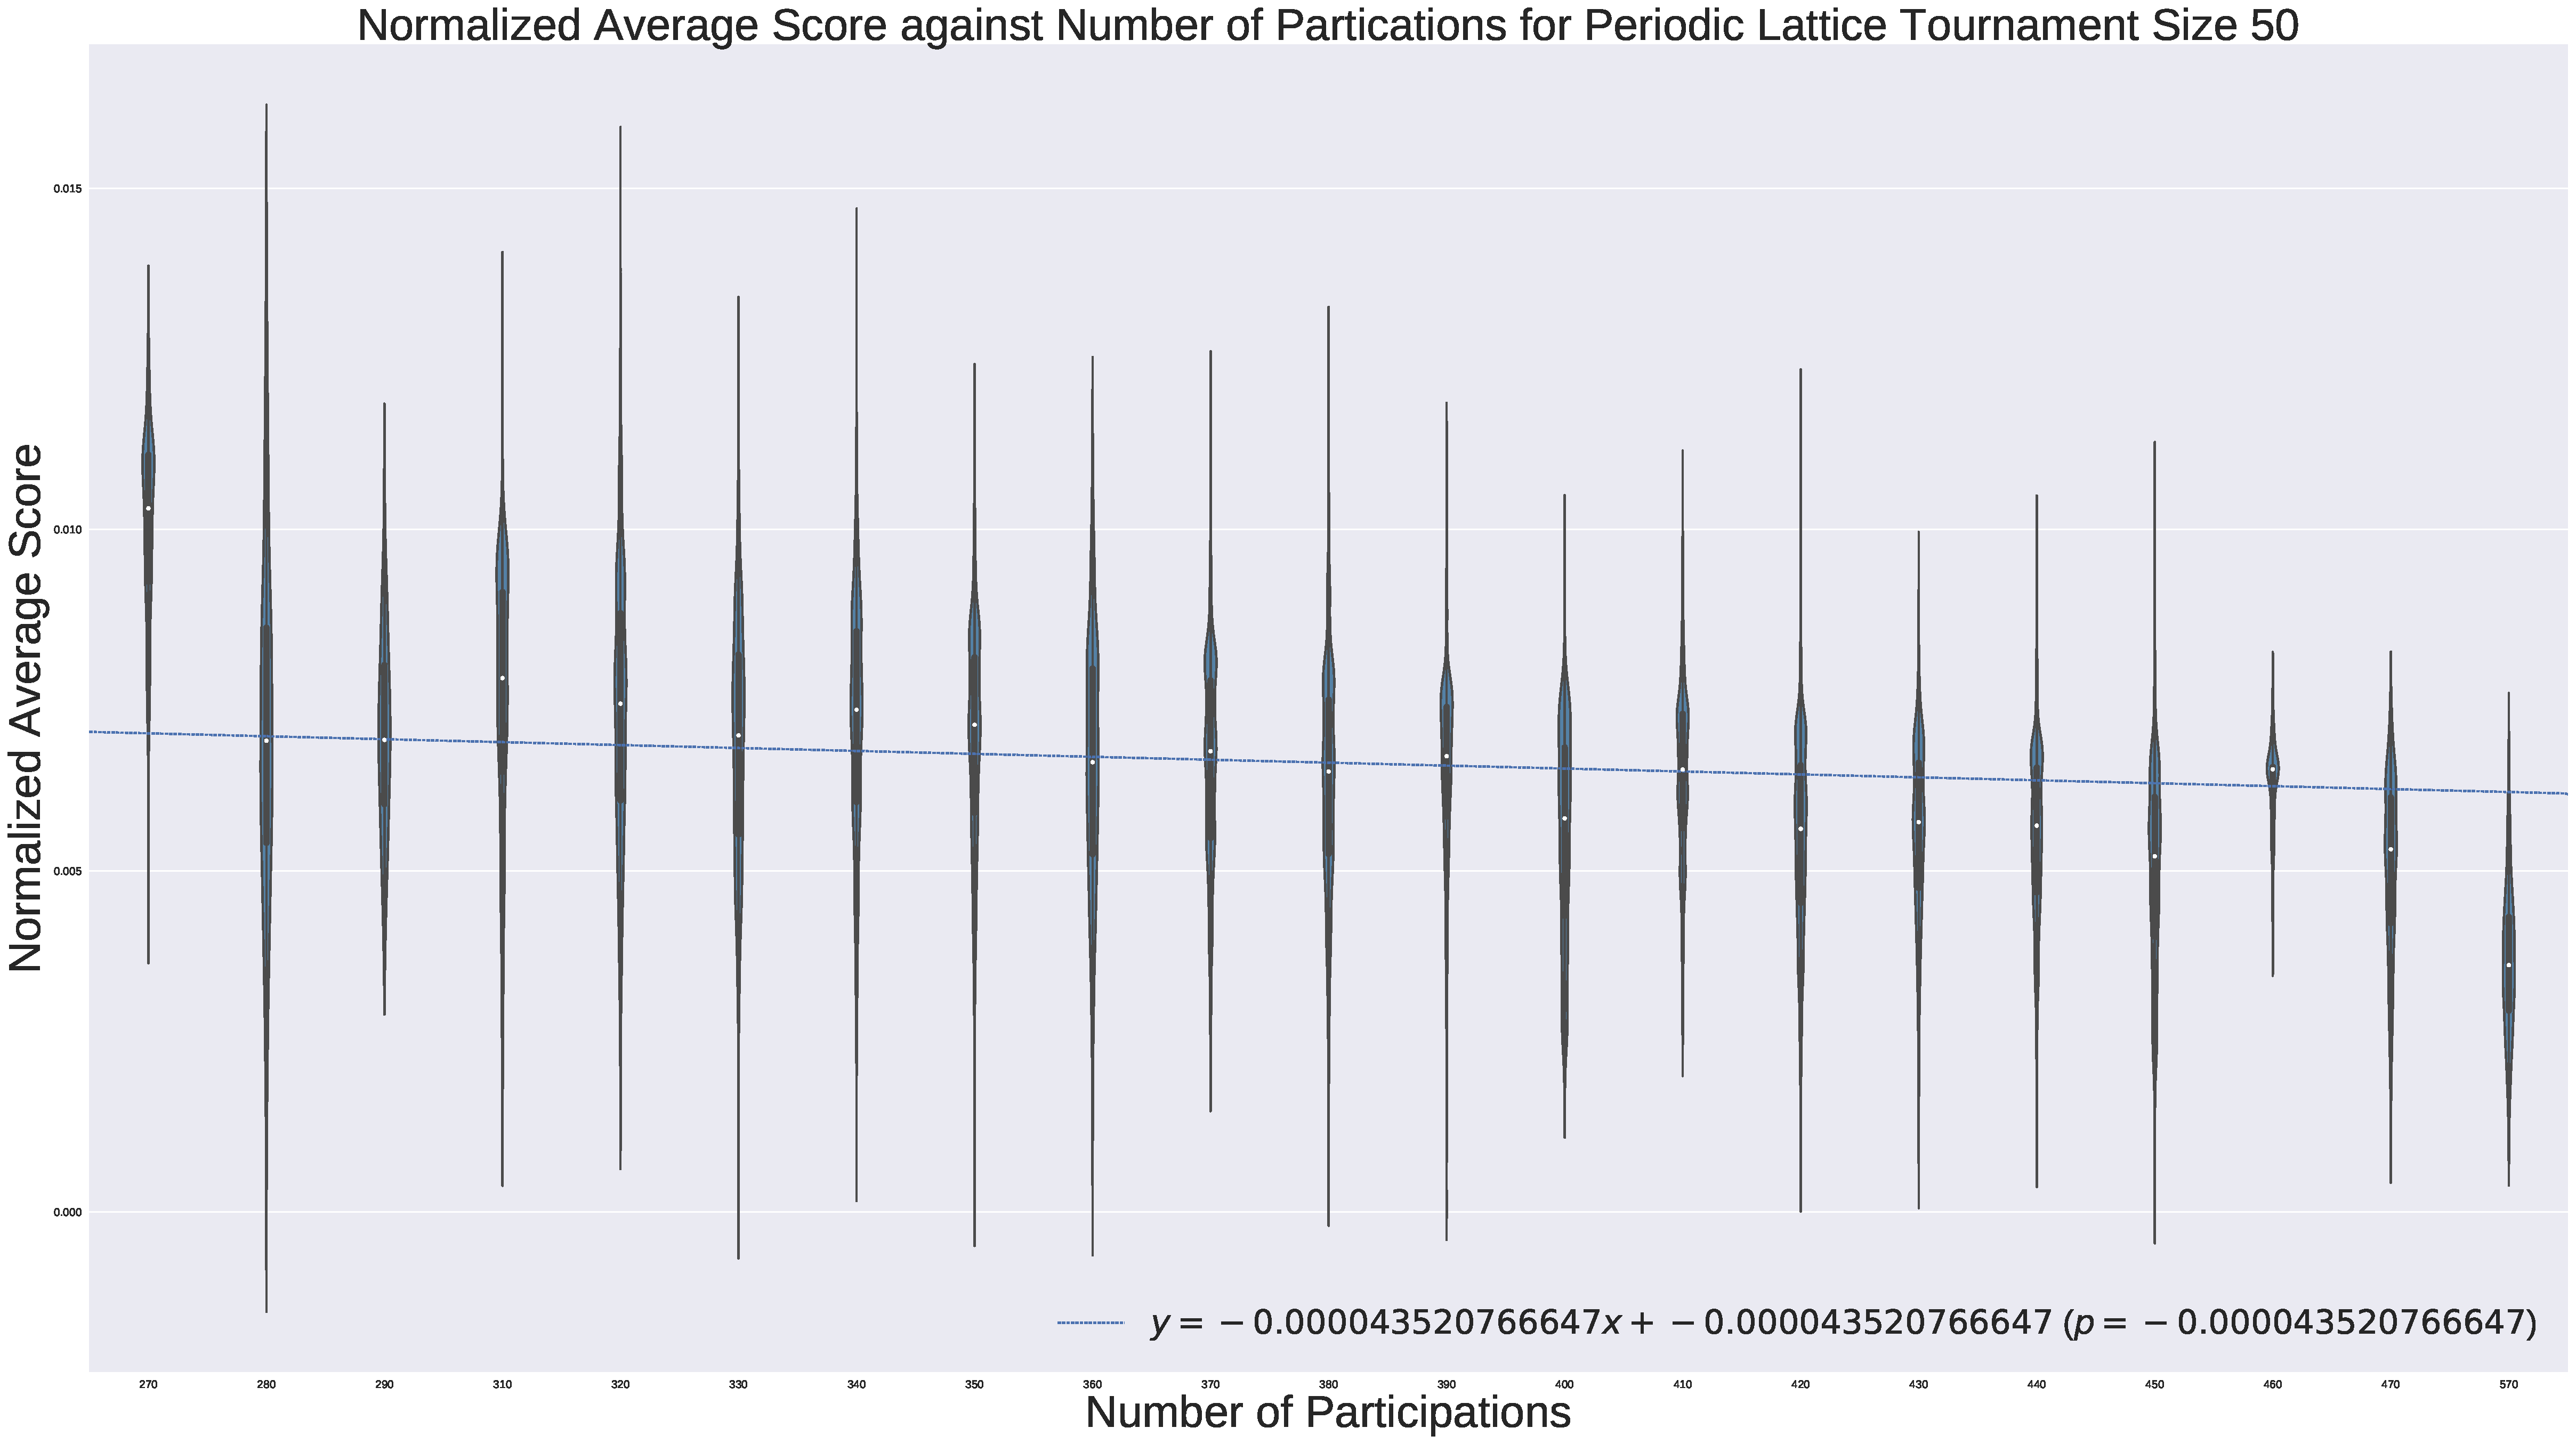
\includegraphics[width=\linewidth]{chapter-three/normalized-score-Periodic-Lattice-50.pdf}
    \caption{Normalized average score cycle s=50.}
    \end{subfigure}
\hfill
    \begin{subfigure}[t]{1\textwidth}\centering
    \centering
        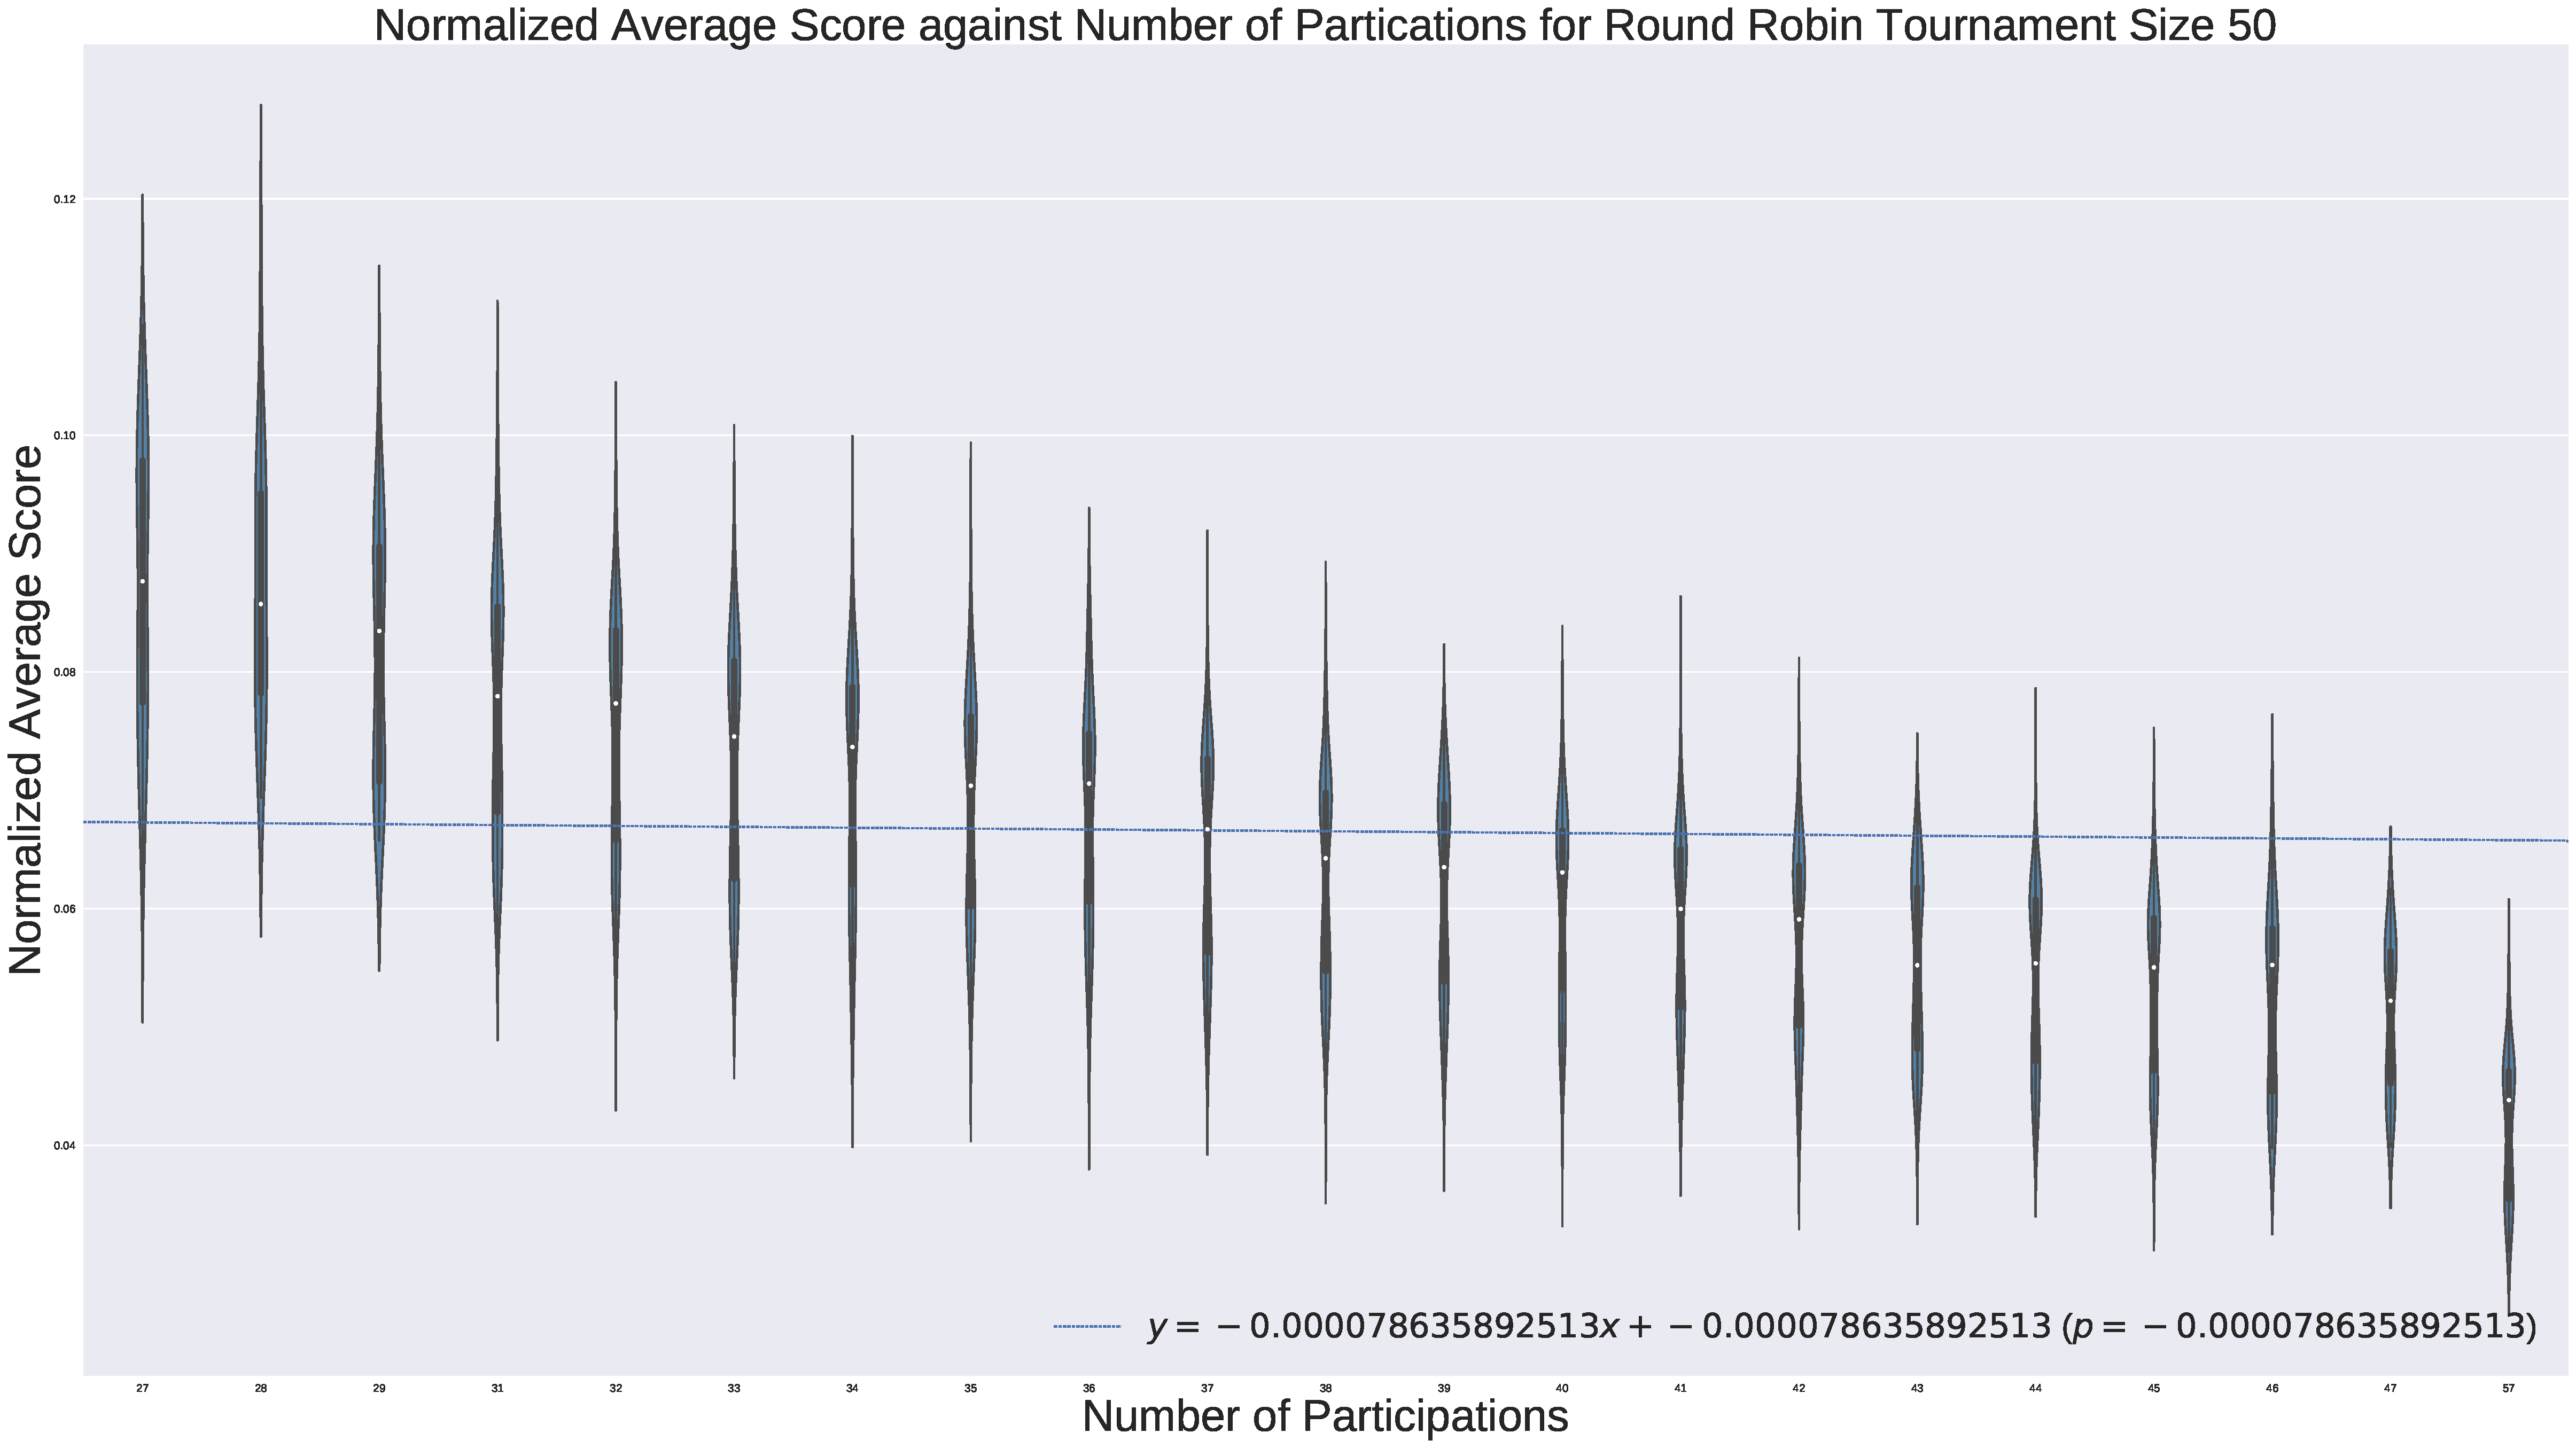
\includegraphics[width=\linewidth]{chapter-three/normalized-score-Round-Robin-50.pdf}
    \caption{Normalized Average Score Round Robin Topology Size 50.}
    \end{subfigure}
\caption{Normalized Average Score for all Three Topologies Size 50.}
\label{fig:average-score-fifty}
\end{figure}

\section{Supplementary Tables}
\section{Strategies List}
\label{append:strategies}
A list of strategies and a simple explanation, on their game play can be found in
Table.
